% Dissertation for Enliang Zheng
% LaTeX template originally obtained from Bjorn B. Brandenburg and Jared Heinly:
% http://www.cs.unc.edu/~bbb/
% http://www.cs.unc.edu/~bbb/diss/unc-dissertation-template.zip
% cvs/proj/v3d/paper-submission/thesis_heinly

% The following definitions are used to build up the lists of advisors/members in the next section of commands.
\def\thesisadvisora{Jan-Michael Frahm}
\def\thesisadvisorb{Enrique Dunn}
\def\thesismembera{Tamara L.~Berg}
\def\thesismemberb{Jojic Vladimir}
\def\thesismemberc{Yaser sheikh}

% The following commands are used throughout the introductory parts of the document.
\def\thesisauthor{Enliang Zheng}
\def\thesisadvisors{\thesisadvisora~and \thesisadvisorb}
\def\thesismembers{\thesisadvisora \\ \thesisadvisorb \\ \thesismembera \\ \thesismemberb \\ \thesismemberc}
\def\thesistitle{Toward 3D reconstruction of static and dynamic objects}
\def\thesistitlepage{Toward 3D reconstruction of static and dynamic objects}

% Control the formatting of the document in various places throughout the common/pages files.
\def\thesisfontsize{12}
\def\thesisleftmargin{1}
\def\thesisrightmargin{1}

\newcommand{\todo}[1]{\ding{110}~\textcolor{red}{TODO: #1}}

% !TEX root = ../thesis_heinly.tex

\documentclass[\thesisfontsize pt,letterpaper,twoside]{report}

% Layout
\usepackage{geometry}
\usepackage{setspace}
\usepackage{titlesec}
\usepackage[subfigure]{tocloft}
\usepackage{etoolbox}
\usepackage{changepage}
\usepackage{indentfirst}
\usepackage[hang]{footmisc}

% Remove the extra space between figures/tables from different chapters in the list of figures/tables.
\makeatletter
\patchcmd{\@chapter}{\addtocontents{lof}{\protect\addvspace{10\p@}}}{}{}{}% List of figures
\patchcmd{\@chapter}{\addtocontents{lot}{\protect\addvspace{10\p@}}}{}{}{}% List of tables
\makeatother

% Citation style
\usepackage{natbib}
\usepackage{apalike}

% include citations inline
\usepackage{bibentry}
\nobibliography*

% Figures
%\usepackage{subfigure}
\usepackage{subfig}
\usepackage{epsfig}
\usepackage{booktabs}
\usepackage{multicol}
\usepackage{listings}
\usepackage{tabu}
\usepackage{enumitem}
\usepackage{algorithm}
\usepackage[noend]{algpseudocode}
\usepackage{caption}
\captionsetup[table]{font={stretch=0.95}}
\captionsetup[figure]{font={stretch=0.95}}

% Math
\usepackage{amsthm}
\usepackage{amsmath}
\usepackage{amssymb}

% Typography
\usepackage{times}
\usepackage{microtype}
\usepackage{textcomp}

% Macro support
\usepackage{xspace}

% Symbols
\usepackage{pifont}

% Color
\usepackage[usenames,dvipsnames]{color}
\usepackage[table]{xcolor}

% PDF links
\usepackage[hidelinks]{hyperref} % backref=page

\renewcommand{\algorithmicforall}{\textbf{for each}}
\def\ForEach{\ForAll}

% !TEX root = ../thesis_heinly.tex

% Use proper margins.
\geometry{letterpaper,left=\thesisleftmargin in,top=1in,right=\thesisrightmargin in,bottom=1in,nohead}

% double-space text
\doublespacing % uses a setstretch of 1.667 for 10pt font, 1.618 for 11pt, and 1.655 for 12pt
%\setstretch{2.0}

\setlength{\footskip}{0.48in}

% Center chapter titles, omit page numbers.
%\titleformat{\chapter}[display]{\fillast\bfseries}{\large\MakeUppercase{\chaptertitlename} \thechapter}{-11pt}{\huge\singlespacing}[\thispagestyle{empty}]
%\titleformat{\chapter}[hang]{\fillast\bfseries}{\large\MakeUppercase{\chaptertitlename~\thechapter:}}{0.5em}{\large}
\titleformat{\chapter}[block]{\filcenter\bfseries\singlespacing}{\MakeUppercase{\chaptertitlename}~\thechapter:}{0.5em}{\uppercase}

\titleformat{\section}{\normalfont\fontsize{12}{15}\bfseries}{\thesection}{1em}{}
\titleformat{\subsection}{\normalfont\fontsize{12}{15}\bfseries}{\thesubsection}{1em}{}
\titleformat{\subsubsection}{\normalfont\fontsize{12}{15}\bfseries}{\thesubsubsection}{1em}{}

% Extend to 2in top margins
% Leave 22pts = 2x font size after heading
\titlespacing{\chapter}{0in}{0.5in}{22pt}

% Indent paragraphs four spaces throughout the thesis/dissertation.
\setlength{\parindent}{4ex}

% Tweak spacing of paragraph labels.
\titlespacing{\paragraph}{0in}{0.08in}{0.07in}

% We want numbered subsubsections
\setcounter{secnumdepth}{3}
\setcounter{tocdepth}{3}

% We need to double-space between footnotes.
\setlength{\footnotesep}{13pt}
\setlength{\footnotemargin}{0.5em}

% We don't want crazy vertical spacing.
\raggedbottom

% We don't want abandoned words.
\clubpenalty=10000 
\widowpenalty=10000

% Prevent awkward hyphenations.
\hyphenation{Raj-kumar}


\input{common/macros}


\usepackage{bm}
\usepackage{bbm}
\usepackage{slashbox}
\usepackage{tabu}
		
\begin{document}

\sloppy % Allow latex to be more "sloppy" in its formatting. This helps reduce words that carry on into the margin.

%\todo{Verify margin dimensions and title spacing throughout the document.}
%\todo{Check for ``Fig.", ``i.e.", ``e.g.", ``etc.", ``?"}
%\todo{Check for ``iconic"}
%\todo{Remove ``I", ``me", ``my", \etc.}

% !TEX root = ../thesis_heinly.tex

% front matter pages use 2in top margin
\newgeometry{left=\thesisleftmargin in,top=2in,right=\thesisrightmargin in,bottom=1in,nohead}
\pagenumbering{roman}

%1. Title Page

% !TEX root = ../thesis_heinly.tex

\begin{titlepage}

\begin{singlespace}
\centering

\currentpdfbookmark{TITLE}{bk:title}

\vspace{1in}
\begin{adjustwidth}{0.5in}{0.5in}
\centering
\MakeUppercase{\thesistitle}
\end{adjustwidth}

\nointerlineskip\vspace{1in}

\thesisauthor

\nointerlineskip\vspace{1in}

\noindent
A dissertation submitted to the faculty of the University of North Carolina at Chapel Hill in partial fulfillment of the requirements for the degree of Doctor of Philosophy in the Department of Computer Science.

\nointerlineskip\vspace{1in}

Chapel Hill\\
\the\year

\end{singlespace}

% Use the following block if you want the committee members to have exactly a 1in margin to the right.
%\nointerlineskip\vspace{0.83in}
%\setlength\topsep{0pt}
%\begin{flushright}
%{
%\setlength{\tabcolsep}{0pt}
%\begin{tabular}[t]{l}
%Approved by: \\
%\thesismembers
%\end{tabular}
%} % large
%\end{flushright}

% Use the following block if you want the committee members to appear approximately 2/3 the way across the page.
\nointerlineskip\vspace{0.71in}
\begin{flushright}
\begin{minipage}{2.1in}
\setlength{\tabcolsep}{0em}
\begin{tabular}{l}
Approved by: \\
\thesismembers
\end{tabular}
\end{minipage}
\end{flushright}

\end{titlepage}


%2. Copyright Page (optional)
\newgeometry{left=\thesisleftmargin in,top=8.42in,right=\thesisrightmargin in,bottom=1in,nohead}

% !TEX root = ../thesis_heinly.tex

\begin{center}
\begin{singlespace}
\copyright \the\year\\
\thesisauthor \\
ALL RIGHTS RESERVED
\end{singlespace}
\end{center}

\clearpage

\newgeometry{left=\thesisleftmargin in,top=2in,right=\thesisrightmargin in,bottom=1in,nohead}

%3. Abstract

% Normal pages from here on out; TOC title takes care of 2in requirement.
\restoregeometry

% !TEX root = ../thesis_heinly.tex

\begin{center}
\vspace*{46pt}
\currentpdfbookmark{ABSTRACT}{bk:abstract}
\textbf{ABSTRACT}
\vspace{4pt}

\begin{singlespace}
\thesisauthor: \thesistitle \\
(Under the direction of \thesisadvisors)
\vspace{10pt}
\end{singlespace}
\end{center}



%3D reconstrcution Recovering 3D information from imagery is an important task in the field of computer vision.
%With the bursting number of images and videos available on the Internet, it has been of interest to the computer vision community to perform 3D reconstruction of a scene from such data for further applications. Though 3D reconstruction, a process that recovers the 3D information of a scene via images, is a traditional topic in computer vision, some of the challenging problems still remain partially solved or even unsolved. This is especially true when using crowd-sourced data with heterogeneous properties, such as images with random occlusions and videos with unknown temporal overlap. Moreover, most existing methods only target the problem of static scene reconstruction, but fail on the dynamic part due to additional challenges such as non-current captures. To push forward the research frontier for image based 3D modeling, this dissertation focuses on the problem of static as well as dynamic object reconstruction from unstructured images or unsynchronized videos. 

The problem of 3D reconstruction from imagery aims at recovering 3D information of a scene based on image colors. Given that a real-world scene typically comprises static scenes (\eg~trees and buildings) as well as dynamic objects (e.g.~, cars and pedestrians), it is of interest to reconstruct both of them for further applications. However, due to many inherent ambiguities in the reconstruction problem, attaining the 3D information with accuracy, robustness, and efficiency is a big challenge. To advance the research frontier for image-based 3D modeling, this dissertation focuses on three challenging problems in static scene and dynamic object reconstruction. 

We first target the problem of static scene depthmap estimation from crowd-sourced datasets. (i.e.~Internect collected photos). While achieving high-quality depthmaps using images taken under a controlled environment is difficult, the task with heterogeneous crowd-sourced data even brings more challenges such as illuminations variance and occasional occlusions. We propose a depthmap estimation method that demonstrates its accuracy, robustness, and scalability on a large number of photos collected from the Internet.
 
Compared to static scene reconstruction, the problem of dynamic object reconstruction from monocular images is fundamentally ambiguous when not imposing any additional assumptions, as having only a single observation of an object is insufficient for valid 3D triangulation (which typically requires multiple concurrent observations). Assuming that dynamic objects of the same class (e.g.~, all the pedestrians walking on a sidewalk) move in a common path in the real world, we develop a method that estimates the 3D positions of the dynamic objects from unstructured monocular images. The experiments on both synthetic and real datasets illustrate the solvability of the problem and the effectiveness of our approach.

Next, we approach the problem of dynamic object reconstruction by using a set of unsynchronized videos that capture the same dynamic event, instead of using monocular images as input. This problem is of great interest because, due to the increased availability of portable capture devices, captures using multiple unsynchronized videos are common in the real world. To resolve the difficulty that arises from non-concurrent captures and unknown temporal overlap among video streams, we propose a self-expressive dictionary learning framework, where the dictionary is defined as the temporally varying structures. The experimental results show that this novel approach solves the previously unsolved problem.


\clearpage


%4. Dedication, Acknowledgement(s) and/or Preface (all optional)

%% !TEX root = ../thesis_heinly.tex

\begin{center}
\vspace*{52pt}
\todo{Dedication: To\dots}
%To all those who have inspired, encouraged, and supported me over the year.
%To all those who have impacted me to be the person I am today.
\end{center}

\pagebreak

% !TEX root = ../thesis_heinly.tex

\begin{center}
\vspace*{46pt}
\currentpdfbookmark{ACKNOWLEDGEMENTS}{bk:acknowledgements}
\textbf{ACKNOWLEDGEMENTS}
\vspace{10pt}
\end{center}

I would like to thank my advisors, Jan-Michael Frahm and Enrique Dunn, for their input and guidance.

I would also like to thank my committee members, Tamara L.~Berg, Vladimir Jojic, and Yaser Sheikh, for their feedback and advice.

Additionally, I would like to thank my labmates, as their company and discussion made my time more fruitful and enjoyable:
Philip Ammirato,
Akash Bapat,
Sangwoo Cho,
Pierre Fite-Georgel,
Yunchao Gong,
Rohit Gupta,
Shubham Gupta,
Xufeng Han,
Jared Heinly
Junpyo Hong,
Yi-Hung Jen,
Dinghuang Ji,
Alex Keng,
Hadi Kiapour,
Hyo Jin Kim,
Wei Liu,
Jie Lu,
Licheng Yu,
Vicente Ord\'{o}\~{n}ez-Rom\'{a}n,
David Perra,
True Price,
Rahul Raguram,
Patrick Reynolds,
Johannes Sch\"{o}nberger,
Meng Tan,
Joseph Tighe,
Sirion Vittayakorn,
Ke Wang,
Yilin Wang,
Yi Xu,
and
Hongsheng Yang.

I would like to thank my parents, who encouraged me to explore, create, tinker, and learn.

Finally, I would like to thank my wife, Lingling Zheng, for her continued support.

\clearpage

%% !TEX root = ../thesis_heinly.tex

\begin{center}
{\Large \textbf{PREFACE}}
\end{center}

ABCDEFGHIJKLMNOPQRSTUVWXYZ
\tbw

\clearpage


%5. Table of Contents, with page references
% !TEX root = ../thesis_heinly.tex

\renewcommand{\contentsname}{\hfill\bfseries\normalsize TABLE OF CONTENTS\hfill}
%\renewcommand{\cfttoctitlefont}{\hfill\Large\bfseries}
\renewcommand{\cftaftertoctitle}{\hfill}
\renewcommand{\cftdotsep}{1.5}
\cftsetrmarg{1.0in}

\setlength{\cftbeforetoctitleskip}{56pt}
\setlength{\cftaftertoctitleskip}{18pt}

% format chapter entries like other entries
\renewcommand{\cftchapfont}{\normalfont}
\renewcommand{\cftchappagefont}{\normalfont}
\renewcommand{\cftchapleader}{\cftdotfill{\cftdotsep}}

\setlength{\cftbeforechapskip}{15pt}
\setlength{\cftbeforesecskip}{10pt}
\setlength{\cftbeforesubsecskip}{10pt}
\setlength{\cftbeforesubsubsecskip}{10pt}

\begin{singlespace}
\currentpdfbookmark{TABLE OF CONTENTS}{bk:contents}
\tableofcontents
\end{singlespace}

\clearpage


%6. List of Tables, with titles and page references (if applicable)

% !TEX root = ../thesis_heinly.tex

\renewcommand{\listtablename}{LIST OF TABLES}
\phantomsection
\addcontentsline{toc}{chapter}{LIST OF TABLES}

\setlength{\cftbeforelottitleskip}{-14pt}
\setlength{\cftafterlottitleskip}{22pt}
\renewcommand{\cftlottitlefont}{\hfill\normalsize\bfseries}
\renewcommand{\cftafterlottitle}{\hfill}

\setlength{\cftbeforetabskip}{12pt}
\cftsetrmarg{1.0in}

\setlength{\cfttabindent}{0in}

\begin{singlespace}
\listoftables
\end{singlespace}

\clearpage


%7. List of Figures or Illustrations, with titles and page references (if applicable)

% !TEX root = ../thesis_heinly.tex

\renewcommand{\listfigurename}{LIST OF FIGURES}
\phantomsection
\addcontentsline{toc}{chapter}{LIST OF FIGURES}

\setlength{\cftbeforeloftitleskip}{-14pt}
\setlength{\cftafterloftitleskip}{22pt}
\renewcommand{\cftloftitlefont}{\hfill\normalsize\bfseries}
\renewcommand{\cftafterloftitle}{\hfill}

\setlength{\cftbeforefigskip}{12pt}
\cftsetrmarg{1.0in}

\setlength{\cftfigindent}{0in}

\begin{singlespace}
\listoffigures
\end{singlespace}

\clearpage


%8. List of Abbreviations (if applicable)
% !TEX root = ../thesis_heinly.tex

\phantomsection
\addcontentsline{toc}{chapter}{LIST OF ABBREVIATIONS}

\begin{center}
\textbf{LIST OF ABBREVIATIONS}
\vspace{16pt}
\end{center}

\noindent
\begin{tabular}{@{}p{0.8in} l}

GMST & Generalized minimum spanning tree \\
NRSFM & Non-rigid structure from motion \\
SfM & Structure-from-motion \\
MRF & Markov Random Field (
%RANSAC & Random sample consensus \\
%SIFT & Scale invariant feature transform \cite{lowe2004_sift} \\
\end{tabular}

\clearpage


%9. List of Symbols (if applicable)
%% !TEX root = ../thesis_heinly.tex

\phantomsection
\addcontentsline{toc}{chapter}{LIST OF SYMBOLS}

\begin{center}
\textbf{LIST OF SYMBOLS}
\vspace{16pt}
\end{center}

\noindent
\begin{tabular}{@{}p{0.8in} l}
$C$ & 3D point co-occurence matrix \\
$C_{ij}$ & Boolean indicating whether 3D points $i$ and $j$ were observed in the same camera \\
$M$ & Number of images \\
$m$ & Number of cameras \\
$n$ & Number of points \\
$O$ & Storage of 3D point observations for each camera \\
$O_i$ & Set of 3D points observed by camera $i$ \\
$O_{ij}$ & Boolean indicating whether 3D point $j$ is observed in camera $i$ \\
$T_i$ & Center position of camera $i$
\end{tabular}

\clearpage


\pagenumbering{arabic}


%%%%%%%%%%%%%%%%%%%%%%%%%%%%%%%%%%%%%%%%%%%%%%%%%%%%%%%%%%%%
%%%%%%%%%%%%%%%%%%%%%%%%%%%%%%%%%%%%%%%%%%%%%%%%%%%%%%%%%%%%

%%%%%%%%%%% Static scene depthmap estimation determines a view-dependent depthfield by leveraging the local photoconsistency of a set of overlapping images observing a common scene. 

\chapter{Introduction}

Imagery records what the world looks like by projecting the 3D scene onto an image plane. However, the 3D information, which depicts the geometry of real objects, is lost during this capture process. Conversely,   3D information is key to many applications, such as augmented/virtual reality \cite{ventura2008depth}, robots and autonomous car navigation \cite{endres2012evaluation}, image-based rendering \cite{View_interpolation1993}, and image enhancement \cite{zhang2014personal}. Moreover, as additional information to RGB (Red, green, and blue) colors, 3D information is leveraged to improve performance of many computer vision tasks such as object classfication/recognition \cite{gupta2013perceptual}  and human pose estimation \cite{CVPR_kinect}. Therefore, there is a strong desire to recover reliable 3D information from 2D imagery.

3D information, when stored in computers, can be represented using 3D point clouds, 3D Polygon meshes or depthmaps. A 3D point cloud is a set of data points in three-dimensional space representing the external surface of an object, and it can be classified as either dense or sparse based on its density. In contrast, a 3D polygon mesh provides additional information in the form of the geometric topology among the 3D points. Compared to these representations which uses values in a global coordinate system, a depthmap is a dense field of depth values indicating the distance of the observed surface relative to a camera. In practice, different representations are adopted according to the requirements of specific applications. 

3D reconstruction from imagery, defined as a process that recovers 3D information from 2D image colors, is a traditional problem in 3D computer vision. Unlike the task of computer graphics that renders 2D imagery from 3D geometry, the inverse process of 3D reconstruction from imagery is more challenging since aiming at recovery of lost information inevitably introduces more ambiguities. Though 3D reconstruction has received heavy study and improved over the last few decades, it still remains a viable research area. This dissertation primarily focuses on the problems of dense static scene reconstruction and sparse dynamic object reconstruction from 2D imagery.

\textbf{Dense static scene reconstruction}.
To attain the 3D information of a static scene, most existing works leverage 2D correspondences and available camera parameters for 3D triangulation. Though camera parameters can typically be estimated by structure from motion or offline calibration methods, obtaining 2D correspondences robustly from image colors still requires further exploration. The 2D correspondences are defined as pixels in different images that observe the same part of a 3D scene. Under the assumption of a Lambertian surface, these 2D correspondences share the same or similar appearances/colors, and hence they have high color consistency.

For each point in one image, finding its correspondence in another image is attained by searching for candidate pixels with best color consistency along a line defined by the 3D geometry (called an epipolar line), and the positions of candidate pixels are determined by depth hypotheses generated in a valid range. Once the correspondence is found, the depth of the corresponding pixel is uniquely determined. However, estimating dense correspondences robustly is difficult since ambiguities arise in the cases of repetitive textures, homogeneous color regions, or occlusions along the epipolar line. 

Recently, there is a growing interest in using the ever-increasing crowd sourced data (\ie~Internet collected photos) for reconstruction, since the large amount of free data has inspired many applications such as virtual photo tours \cite{Snavely2} and image enhancement \cite{zhang2014personal}. With the non-controlled imagery as input, finding 2D correspondences based on colors is more challenging due to a diversity of factors such as heterogeneous resolution and scene illuminations, unstructured viewing geometry, scene content variability and image registration errors. To address these issues, it is normally assumed in the massive number of images, there are a subset of images sharing similar image characteristics. Therefore, determining a suitable subset of images or pixels for correspondence search becomes essential \cite{Goesele07}.

Dense reconstruction typically has very high computational complexity, since the traditional process involves exhaustive evaluations of a large number of depth hypotheses \cite{yang2003multi}. The increasing availability of crowd-sourced datasets has explicitly brought efficiency and scalability to the forefront of application requirements.  Moreover, the high complexity of a method would impede its usage in less-powerful electronic devices such as smart phones. To this end, there is a compelling demand to develop efficient and scalable methods for dense reconstruction.

\textbf{Sparse dynamic object reconstruction}.
The problem of dynamic object reconstruction specifically aims at 3D reconstruction under the circumstance of non-concurrent image captures. To be more precise, the dynamic object is only observed by one image at each time instance. This poses an additional challenge compared to the problem of static  scene reconstruction, since 3D triangulation becomes invalid and impossible with the unitary observation, even assuming 2D correspondences among non-concurrent images are correctly found. Given a unitary observation, it is only known the 3D point lies somewhere along the viewing ray determined by the 2D meansurement and the camera pose, but the depth along the viewing ray cannot be easily computed. Primarily due to this intrinsic difficulty, the state of the art for dynamic object reconstruction falls far behind that of static scene reconstruction.

The problem of dynamic object reconstruction is fundamentally under-constrained and requires further assumptions. Many existing works make various assumptions on scene geometry, object motion, capture pattern, \emph{etc}. For instance, most non-rigid structure from motion (NRSFM) methods assume the 3D shapes of deforming objects lie in a low dimensional subspace, and hence any shape can be represented as a linear combination of $K$ shape bases \cite{Bregler_CVPR2000,torresani2008nonrigid,dai2014simple}. Trajectory-based methods assume smooth motion of the dynamic objects across time \cite{Akhter_NIPS08}. \citet{bao2011toward} assume a non-coplanar layout of objects and cameras, plus a prior knowledge of the object size. \citet{Hoiem_CGRAPH2005} assume the scene only consists of the elements of sky, ground plane, and vertical buildings facades. When developing methods for dynamic object reconstruction, in addition to making valid assumptions, having fewer but more general assumptions is vital to enable the methods to work more universally and robustly in real scenarios. 

Trajectory triangulation -- one kind of dynamic object reconsturction problems -- computes the trajectory of a dynamic 3D point given a set of unitary observations across time. Under the assumption of smooth object motion and available sequencing information (\ie~the temporal order of images being taken), existing method can achieve accurate reconstruction results \cite{Park_ECCV2010,Valmadre_CVPR2012}. Although the assumption of smooth object motion is typically true for real dynamic objects, in practice easily obtaining the sequencing information and achieving high reconstruction accuracy cannot be satisfied simultaneously \cite{ZhuCL_CVPR11,Valmadre_CVPR2012}. The sequencing information tells that a moving 3D point is spatially close, if the temporal stamp of two capturing images are close. In effect, it is this spatial proximity that is leveraged by the existing methods \cite{Park_ECCV2010,Valmadre_CVPR2012} for reconstruction. In contrast, our research focuses on 3D reconstruction of dynamic objects given no or partial information of the spatial/temporal proximity.

%%%%%%%%%%%%%%%%%%%%%%%%%%%%%%%%%%%%%%%%
\section{Thesis Statement}
Robust and efficient depthmap estimation for Internet collected photos is attained through a framework of joint view selection and depthmap estimation, and accurate dynamic object reconstruction from unstructured images or unsynchronized videos is achieved given no or partial information of spatial/temporal proximity.

%%%%%%%%%%%%%%%%%%%%%%%%%%%%%%%%%%%%%%%%
\section{Outline of Contributions}
This dissertation contributes significantly to advance the state-of-the-art techniques for the problems of static scene reconstruction and dynamic object reconstruction, and it builds on our published works \cite{zheng2014patchmatch,zheng2014joint,zhengiccv_2015}.

\begin{description}

\item[PatchMatch Based Joint View Selection and Depth Estimation:]
Chapter \ref{ch:patchmatch} focuses on the problem of depthmap estimation using Internet collected photos. The non-controlled input imagery presents practical challenges such as heterogeneous scene illuminations and unstructured viewing geometry. Therefore, it is vital to determine a subset of images or pixels in the dataset for robust depth estimation. Moreover, the ever-increasing number of crowd-sourced datasets have explicitly brought efficiency and scalability to the forefront of application requirements.

To solve this problem, we propose a probabilistic framework for joint view selection and depth estimation at the pixel level. Our new method attains more complete depthmaps compared to the state-of-the-art method for Internet collected photos \cite{Goesele07}. To increase the efficiency and scalability, our framework seamlessly incorporates the PatchMatch scheme \cite{patchMatchStereo1} to  reduce the size of the depth hypotheses set. Also, the memory requirement of our framework scales linearly with respect to the number of source images, as opposed to exponentially \cite{CombinedDepthOutlier}. Moreover, our method is designed to process each row or column of the reference image independently, enabling easy parallelization and GPU implementation.

\item[Joint Object Class Sequencing and Trajectory Triangulation:]
Chapter \ref{ch:jost} targets the problem of reconstructing the 3D positions of dynamic objects from a set of unstructured images. Each dynamic object is observed by the images once so that the traditional 3D triangulation for static scenes is impossible. To tackle the fundamentally under-constrained problem, we assume that all of the objects of the same class (\eg~pedestrians or cars) move in a common path in 3D space. Then, our method estimates the 3D positions of the dynamic objects by triangulating the trajectory formed by all the objects moving in the common path. 

To the best of our knowledge, no current methods have solved this challenging problem. 
Our method uses the object detection outputs as a general feature for each dynamic object, as opposed to typical image features such as points or edges. In solving the problem, recovering the sequencing information, which is defined as the topology of the trajectory in this specific problem, is vital for trajectory triangulation. We propose to jointly estimate the sequencing information and the 3D points, which is posed as minimizing a nonconvex function. To minimize the function, we propose a novel discrete-continuous optimization approach based on the generalized minimum spanning tree (GMST). 

\item[Dynamic Object Reconstruction from Unsynchronized Videos:]
Chapter \ref{ch:video_l1} aims at the similar problem of dynamic object reconstruction, but using unsynchronized video streams as input. To handle this unconstrained problem, we observe that any shape at one time instance is a linear combination of other shapes (self-expression), under the assumption of smooth object motion. The problem is then solved by learning a self-expressive dictionary, which is defined as a collection of temporally varied structures. 

The main contribution of this paper is solving the new problem of dynamic object reconstruction without temporal order information across video streams (also called sequencing information). This is contradictory to the existing works that strictly rely on available sequencing information \cite{Park_ECCV2010,Valmadre_CVPR2012}. 
Moreover, to the best of our knowledge, we are the first to use the self-expression prior for dynamic object reconstruction. This prior has the potential to be used in the traditional non-rigid structure from motion (NRSFM) problem, where most existing methods use the assumption that any shape is a linear combination of $K$ fixed shape bases \cite{dai2014simple,Bregler_CVPR2000}. In learning the dictionary, we propose an efficient solver based on the alternating direction method of multipliers (ADMM) \cite{boyd2011distributed}.

\end{description}

Each of these contributions addresses the issue of 3D reconstruction from 2D imagery. The next three chapters describe each method in detail, and Chapter \ref{ch:discussion} concludes the dissertation with potential extensions to our works and possible future research directions. 



%%%%%%%%%%%%%%%%%%%%%%%%%%%%%%%%%%%%%%%%%%%%%%%%%%%%%%%%%%%%
%%%%%%%%%%%%%%%%%%%%%%%%%%%%%%%%%%%%%%%%%%%%%%%%%%%%%%%%%%%%
\chapter{Related work}

3D reconstruction from 2D imagery has been studied intensively and extensively by many researchers in the computer vision community. In this section, I first review the works for camera parameter estimation, and then survey the works related to static and dynamic object reconstruction respectively.

\section{Camera parameter estimation}
Camera parameters are generally considered as an prerequisite for 3D reconstruction, since they provide the geometric relationship among different cameras. For instance, with this geometric information, the mapping from a 3D point to an image pixel can be uniquely determined.
Being as two parts of the camera parameters, the internal (intrinsic) part has focal length, principle point, skew parameter, and radial distortion that convert the space coordinates to image coordiantes, the external (extrinsic) part describes a camera's rotation and translation relative to a global coordinate system \cite{Hartley2004}. 

Given the importance of camera parameters in computer vision tasks such as 3D reconstruction, lots of works have been done for camera parameters estimation, a process also called camera calibration. Earlier works for camera calibration require a calibration object such as a planar checkerboard to be seen by the cameras \cite{conf/cvpr/SturmM99,zhang2000flexible,caltoolbox}, which impose a significant constraint in its application. Thanks to the recent development of techniques in structure from motion (SfM) \cite{Snavely2,snavely2008modeling,WuVSFM,wilson2013network,heinly2014_duplicate_structure,schoenberger2015paige,Heinly,heinly_dissertation,zheng2015_structureless_resection}, camera calibration can be achieved by just leveraging 2D correspondences among multiple images. 

Structure from motion is a pipeline that targets estimating the cameras parameters of the images that share the same observations of a static scene. A typical pipeline includes the main steps of feature extraction \cite{lowe2004_sift,rublee2011_orb,bay2008_surf}, inlier correspondence searching \cite{raguram2013usac}, camera pose estimation \cite{nister2003_five_point,kneip2011novel,zheng2014general,zheng2015_structureless_resection} and bundle adjustment \cite{agarwal2010_ba,wu2011_multicore_ba}. Recent works  in structure from motion has exhibited its accuracy, efficiency and robustness to be applicable in most real scenarios.


%While structure from motion estimates camera parameters and produce a sparse 3D point cloud of a static scene, it is the task of stereo that builds a dense model.

\section{Static scene reconstruction}
As a main research subject in 3D computer vision, there are a ton of works addressing issues in static scene reconstruction. Early works mainly focus on depthmap estimation on binocular images \cite{boykov2001fast,Sun_ECCV2002_stereoBeliefProp,scharstein2002taxonomy,scharstein2007learning}. The two images are typically rectified so that searching the correspondence of a pixel is executed on the same line in another image. In contrast, multiview depthmap estimation (MVDE) use multiple images to reduce the ambiguity when searching correspondences. Moreover, the redundant information in the estimated multiple depthmaps can be leveraged to filter out wrongly estimated depth. %This step, called depthmap fusion, is also referred as a process to fuse depthmaps into a unified mesh model. 
This section first discusses the most related works for multiview depthmap estimation and the associated issues such as the robustness and the efficiency, and then discusses briefly the methods generating a consistent point cloud or mesh.

\subsection{Multiview depthmap estimation}
Handling occlusion is important in depthmap estimation, and it firstly emerged in two view stereo \cite{Sun_ECCV2002_stereoBeliefProp, Sun_CVPR2005_stereo, Xiao:2008}. However, in these methods, the occluded pixel region is only marked with unknown depth due to the unavailable correspondence in another image. 

In principle, the additional view  redundancy available to MVDE can be leveraged to resolve occlusions. \citet{handle_occlusion2001} explicitly address occlusion in multi-baseline stereo by only using the subset of the heuristically selected overlapping cameras with the minimum matching cost. The heuristic provides occlusion robustness as long as there is a sufficient number of unoccluded views (typically 50\%). \citet{MultiHypothesis_ECCV2008} choose the best few depth hypotheses for each pixel, following with a MRF optimization to determine a spatially consistent depthmap. Their method chooses source images based on spatial proximity of cameras. \citet{Strecha_BayesModelCVPR2004} handle occlusion in wide-baseline multi-view stereo by including visibility within a probabilistic model, where the depth smoothness is enforced on neighboring pixels according to the color gradient. The work of \citet{Strecha_BayesModelCVPR2004} is further extended in \citet{CombinedDepthOutlier} where the depth and visibility are jointly modeled by hidden Markov random fields. In \citet{CombinedDepthOutlier}, the memory used for visibility configuration of each pixel is $2^K$, which grows exponentially with respect to the number of input images $K$. Hence, the approach is limited to very few images (three images in their evaluation). In contrast, our memory usage is linear with the number of images $K$. %Comparing to above methods, our approach is far more scalable in terms of its source image capacity. This scalability is essential when dealing with large datasets such as internet photo collections.
\citet{Gallup08} present a variable-baseline and variable-resolution framework for MVDE, exploring the attainment of pixel-specific data associations for capture from approximately linear camera paths. While that work illustrates the benefits of fine grain data association strategies in multi-view stereo, it does not easily generalize to irregularly captured datasets. %Internet photo collection as targeted by our proposed method.

Given the redundant information among multiple depthmaps,
lightweight depthmap fusion removes outlier depth by leveraging the mutual depth consistency among multiple depthmaps. 
\citet{Shen_TIP2013} computes the depthmap for each image using PatchMatch \mbox{stereo}, and enforces depth consistency over neighboring views. \citet{LeastCommitment_3DIMPVT2012} follows a scheme similar to Camppbell \citet{MultiHypothesis_ECCV2008} but select the final depth through a process enforcing mutual consistency across all depthmaps. These methods require the depthmaps of other views to be available, while in contrast we aim at developing a method that directly outputs an accurate depthmap. 

%

\subsection{Robustness}
Robust stereo performance for crowd sourced data is an ongoing research effort.
%Due to the irregular spatial distribution and illumination aberration for Internet photo collections in general, a small set of images may not be sufficient for depth estimation, and determining data associations for depth estimation is a more difficult task.
%\citet{Frahm2010} discern a suitable input datum by using appearance clustering using a color augmented GIST descriptor \cite{oliva2001modeling} along with feature-based geometric verification.
%\todo{cite jared}
Images downloaded from Internet (such as Flickr\footnote{https://www.flickr.com/} or Panoramio\footnote{http://www.panoramio.com/}) by searching key words are unstructured imagery with a large portion of unrelated images. To discern a suitable input datum for stereo, \citet{Frahm2010}  use appearance clustering of a color augmented GIST descriptor \cite{oliva2001modeling} along with feature-based geometric verification. In contrast, \cite{Heinly} discover the image relationship by proposing a streaming paradigm that register images to a vocabulary tree built online. However, even the unrelated images are purged, using the data for stereo is still challenging due to the heterogeneous capture characteristics.

To estimate the depthmap of a image, \citet{Frahm2010} select the most related images based on the number of sparse feature points shared in common. The depthmap is estimated using the heuristic K-best planesweeping algorithm proposed by \cite{handle_occlusion2001}. Due to the issues such as illumination difference and occlusion, their estimated depthmaps are of low quality. 
\citet{InternetScaleMVS_CVPR2010} use structure from motion (SFM) to purge redundant imagery but retain high resolution geometry. Their iterative clustering merges sparse 3D points and cameras based on visibility analysis. Although intra-cluster image partitioning is not performed, the cluster size is limited in an effort to maintain computational efficiency. \citet{Goesele07} address the viewpoint selection for crowd sourced imagery by building small size image clusters using the cardinality of the set of common features among viewpoints and a parallax-based metric. This image-wide selection may not be robust to outlier pose estimates. After this, images are resized to the lowest common resolution in the cluster. Pixel depth is then computed using four images selected from the cluster based on local color consistency.

\subsection{Efficiency}
Efficiency is an important issue in depthmap estimation. Traditional methods on large baseline stereo generally involve exhaustive evaluations of a large number of depth hypotheses. The high complexity of computation is not only time-consuming \cite{yang2003multi,CombinedDepthOutlier,Gallup07,LeastCommitment_3DIMPVT2012}, but also prohibitive in less powerful devices such as smart phones. 

The recently proposed PatchMatch is an efficient sampling scheme. Though the scheme has no strict theory or proof of its working mechanism, it has been empirically shown that it always works very well in practice. The PatchMatch was firstly proposed to find approximate nearest neighbor matches between image patches in \citet{Barnes:2009:PAR}, and later \citet{patchMatchStereo1} introduce it to solve the two view stereo problem. PatchMatch initializes each pixel with a random slanted plane at random depth, and is followed by the propagations. The nearby and the current pixels' slanted planes are tested and the one with the best cost is kept. \citet{patchMatchStereo2} combine the PatchMatch sampling scheme and belief propagation to infer an MRF model that has smoothness constraints.
%By combining guided filter and PatchMatch, Lu \etal \cite{PMF_Hongsheng} provide an efficient edge-aware filtering for correspondence field estimation, which can be applied in two view stereo.
While the original PatchMatch stereo was a sequential method, \citet{patchMatchParallel} parallelize the algorithm by restricting the propagations to only horizontal and vertical directions. Our research further explore the potential of the PatchMatch in wide baseline stereo with large hypotheses space.

\subsection{Point cloud and mesh generation}
By far, we only discuss the works focusing on depthmap estimation. Some other methods aim at generating a consistent 3D model (either point cloud or mesh) instead of depthmaps. 
\citet{FURUKAWA_PAMI2010} aim at densifying the sparse point cloud from feature triangulation.
They present an accurate Patch-based MVS approach that starts from a sparse set of matched keypoints, which were repeatedly expanded until visibility constraints are invoked to filter out false matches. 
\citet{Zaharescu_PAMI2011} propose a mesh evolution framework based on a new self-intersection removal algorithm. 

A typical way for 3D mesh generation is to fuse the depthmaps into a consistent model by leveraging the redundant information across images. \citet{gallup20103d,gallup2010heightmap} develop heightmap-based fusion methods that work well for planar object surfaces such as building facades. \citet{zach2008fast} tackles the surface reconstruction task in a variational formulation.
Given that all these methods are volumetric-based and memory inefficient, \citet{zheng2012efficient} instead propose to compress the volume of interest by Haar wavelet, and hence much less memory is required. \citet{JAN} propose a method that reconstructs surfaces that do not have direct support in the input 3D points by exploiting visibility in 3D meshes. Their method has been shown to work pretty robustly on the regions with less texture.


\section{Dynamic object reconstruction}
The following sections outline the related works of trajectory triangulation, image sequencing, non-rigid structure from motion (NRSFM), and single-view reconstruction.

\subsection{Trajectory triangulation}
%Trajectory triangulation estimates the 3D points of dynamic objects given a sequence of images\cite{avidan2000trajectory,Park_ECCV2010,Valmadre_CVPR2012,ZhuCL_CVPR11,park20153d}.
\citet{avidan2000trajectory} first coined the task of trajectory triangulation, which is defined as  reconstruction of a moving point from monocular images. That is, each dynamic point is observed by only one camera at a time. Their method assumes the dynamic point moves along a simple parametric trajectory, such as a straight line or a conic section. Apparently, this is a rather strict constraint to impede its application in real scenarios. 
In contrast, some other methods  \cite{Park_ECCV2010,Valmadre_CVPR2012,ZhuCL_CVPR11,park20153d} focus on a more general model by only assuming a smooth motion of dynamic objects.

\citet{Park_ECCV2010} represent the trajectory with a linear combination of low-order discrete cosine transform (DCT) bases, and the trajectory is triangulated by estimating the coefficients of the linear combination.
There are two fundamental limitations of their method as observed in  \citet{Valmadre_CVPR2012}.
First, there is no automated scheme to determine the optimal number ($K$) of DCT bases.
Second, the correlation between the object trajectory and the camera motion inherently limits the reconstruction accuracy.
To overcome the first limitation, \citet{park20153d} select $K$ by checking the consistency of the reconstructed trajectory in an N-cross validation scheme.
Alternatively, \citet{Valmadre_CVPR2012} propose a new method without using DCT bases. They estimate the trajectory by minimizing the trajectory's response to a bank of high-pass filters.
To overcome the second limitation,
\citet{ZhuCL_CVPR11} propose to incorporate the 3D structures of a number of key frames to enhance the reconstructability. However, obtaining those key-frame 3D structures requires manual interaction. 
All the methods \cite{Park_ECCV2010,Valmadre_CVPR2012,ZhuCL_CVPR11} require the sequencing information of the images, 
but in natural capture setups, the availability of sequencing information and high reconstructability typically cannot be fulfilled simultaneously \cite{ZhuCL_CVPR11,park20153d}. 

%Zheng \etal~\cite{zheng2014joint} address a slightly different problem. They triangulate the object class trajectory, which is defined by the connection of the objects of the same class moving in a common 3D path, from a collection of unordered images. Their method jointly estimates the trajectory and sequencing, but has low scalability and efficiency due to the NP-hard GMST problem. In contrast, our proposed method reconstructs the dynamic objects without sequencing information across videos.

%Recently, Vicente \etal \cite{vicente2014reconstructing} introduced a dense reconstruction approach from unordered image sets leveraging manual object segmentation and semantic labeling for objects contained in the PASCAL-VOC dataset. Their method relies on the fact that similar objects of the same class in a similar pose are visible within the dataset. In contrast, our proposed method reconstructs the object shape without requiring the presence of similar object shapes in the dataset or leveraging semantic information to enable the reconstruction. Russell \etal \cite{russell2014video} introduce a monocular video based reconstruction method, which relies on hierarchical segmentation of a scene into objects, object parts, and background, in order to successfully reconstruct the scene. This approach assumes a known temporal ordering of the video frames and only considers a single camera's information. Our proposed method does not require known temporal ordering and leverages all available observations.

\subsection{Sequencing and Synchronization}
Sequencing information is important in trajectory triangulation. Recently,
\citet{Basha_ECCV2012, Basha_ICCV2013} target the problem of determining the temporal order of a collection of photos without recovering the 3D structure of the dynamic scene. The method in \citet{Basha_ECCV2012} relies on two images taken from roughly the same location to eliminate the uncertainty in the sequencing. \citet{Basha_ICCV2013} later introduce a solution that leverages the known temporal order of the images within each camera. Both of these methods assume dynamic objects move closely to a straight line within a short time period, but in practice, points can deviate considerably from the linear motion model, especially when the temporal discrepancy between images is large. 

Video synchronization has attracted much attention in the computer vision community \cite{Tuytelaars_CVPR,shrestha2010synchronization,rao2003view}. Those methods have various constraints such as camera motion, availability of sound, and number of videos. 
%While our approach aims at dynamic 3D reconstruction without sequencing, the local temporal order can be recovered as a byproduct of our approach. 

\subsection{Articulated object reconstruction}
%As another class of reconstruction, 3D articulated object reconstruction given monocular image sequences has received much attention. 
%Several particle filter %approaches have been developed for 3D human tracking [27, 26]. Wei et al. [32]
%and Valmadre et al. [31] reconstruct the 3D human poses from a small number of2D point correspondences obtained from uncalibrated monocular images. 
Trajectory triangulation suffers from the reconstructability problem of inaccurate reconstruction if the camera motion is relatively smaller than the object motion \cite{park20153d}. 
In the case of 3D reconstruction of articulated objects, we can enforce an additional constraint that the distances between joint points (according to the topology) are fixed, which helps to reduce ambiguities in reconstruction. 
Based on the previous work by \citet{Park_ECCV2010}, the authors further reconstruct 3D articulated motion with the constraint that a trajectory remains at a fixed distance with respect to a parent trajectory \cite{Park_ICCV2011}. Their work shows the improvement of the reconstructibility over their earlier approach \cite{Park_ECCV2010}.
However, the formulation involves solving an NP-hard quadratic programming problem, which is intractable in the case of a large number of input images. 
To conquer the limitation, \citet{Valmadre_ECCV2012} develop a dynamic programming approach that is guaranteed to solve the problem in a timely manner. 
As opposed to articulated object reconstruction, our research focuses on reconstructing more general dynamic objects. 

\subsection{Non-rigid SfM}
One class of related works solve the non-rigid structure from motion (NRSFM) problem, which targets simultaneous recovery of camera motion and 3D structure using an image sequence. These methods typically start from a set of 2D correspondences across frames. 
As an important extension of the well-known Tomasi-Kanade factorization \cite{tomasi1992shape}, 
the work by \citet{Bregler_CVPR2000} tackles the NRSFM problem through matrix factorization, with the assumption that deforming non-rigid objects can be represented by a linear combination of low-order shape bases. 
%It was later shown that in order to achieve a unique solution, more than just the orthogonality constraints have to be used~\cite{Xiao_ECCV2004}. To solve the ambiguity, prior knowledge is required to obtain a unique solution. 
It is later shown by \citet{Xiao_ECCV2004} that utilizing only orthogonality constraints on the camera rotation is not enough, and a basis prior is required to uniquely determine the shape bases.
%In the same spirit, various priors on the shape basis or shape coefficients have been introduced \cite{torresani2008nonrigid}.
However, \citet{akhter2009defense} discover that though the ambiguity in the shape bases is inherent, the 3D shape itself can be uniquely recovered without ambiguity.
Not until very recently, \cite{dai2014simple} propose a new prior-free method that estimates the shape matrix without explicitly recovering the shape bases, which is achieved by minimizing the nuclear norm of the shape matrix.

As a dual method to the above shape-based methods, \citet{Akhter_NIPS08} propose the first trajectory-based NRSFM approach, which leverages DCT bases to approximately represent object point trajectories.
While shape-based approaches typically do not require sequencing information,  trajectory-based approaches completely fail if image frames are randomly shuffled \cite{dai2014simple}.

At first glance, it seems that the NRSFM problem targets a more complete problem than that of trajectory triangulation since the former additionally assumes unknown camera poses as opposed to the latter.
However, these approaches assume orthographic or weak perspective camera models, and it has been shown empirically that the extension of these methods to the projective camera model is not straightforward \cite{Park_ECCV2010}. There are works for projective non-rigid shape and motion recovery based on tensor estimation \cite{hartley2008perspective,vidal2006nonrigid}, but this challenging problem is still under on-going research. Moreover, the NRSFM methods only recover the shape of the object without absolute translation due to the inherent ambiguity arising from the unknown shape translation and the unknown camera translation. 

%In contrast, our approach aims for solving the non-rigid structure from motion problem by leveraging unordered trajectories observed by perspective cameras.
%He \etal \cite{YuchaoDai_CVPR2012} proposed a prior-free solution to the non-rigid structure from motion problem for orthographic cameras which does not require any known temporal relations. However, in order to succeed, they require known ordered trajectories. In contrast, our proposed method does not require ordered trajectories.

%Another related class of methods are the approaches for articulated object reconstruction from monocular videos and images sequences.
%Urtasun \etal \cite{Urtasun_CVPR2006} use Gaussian Process Dynamical Models (GPDMs) to learn human pose and motion priors for 3D people tracking.
%With Bayesian model averaging, a GPDM can be learned from relatively small amounts of data, and it generalizes gracefully to motions outside the training set.
%A popular class of approaches are the particle filter based 3D tracking methods \cite{SminchisescuT_CVPR2003, Sidenbladh_ECCV2000}.

%Tuytelaars \etal~\cite{Tuytelaars_CVPR} propose a method to automatically synchronize two video sequences of the same event. They do not use any constraints from the scene or cameras, but rather rely on point correspondences among the video sequences.

%Unsupervised dictionary learning has also been widely used for reconstructing noisy signals and is closely related to our proposed framework. 
%Along these lines, Mairal \etal~\cite{Mairal_PAMI} show that better results can be obtained when the dictionary is tuned to the specific task.
%In~\cite{Mairal_NIPS} the authors further observe that using sparse coding to the problem of dictionary learning can reduce storage and computational requirements, as well as obviate the need of an explicit learning rate tuning.

%Tuytelaars \etal~\cite{Tuytelaars_CVPR} propose a method to automatically synchronize two video sequences of the same event. They do not use any constraints from the scene or cameras, but rather rely on point correspondences among the video sequences. Wedge \etal \cite{wedge2005_cvpr} propose an efficient coarse-to-fine approach for synchronizing two video sequences recorded at the same frame rate by stationary cameras with fixed internal parameters. In contrast to these methods, we propose a framework for the temporal alignment of multiple video sequences with arbitrary capture characteristics. After briefly discussing related work, we now proceed to provide the notation and intuitions behind our proposed method.


\subsection{Single image reconstruction}
While trajectory triangulation and NRSFM estimate 3D points from an image sequence, some other works target the problem of 3D reconstruction from a single image. Since there is only one shot of the object, the object motion, either static or dynamic, becomes irreverent for the reconstruction. 

Some works focus on 3D reconstruction of Manhattan world \cite{Coughlan_ICCV99}, which is defined as
man-made scenes with mainly orthogonal facades. In this scenario, 3D reconstruction from a single image can be simplified to finding 3D lines and planes within the scene. The work by \citet{Delage_ISRR2005} uses a MRF model to identify the different planes and edges in the scene, as well as their orientations. Then, an iterative optimization algorithm is applied to infer the planes' positions. \citet{Ram_ICCV2013} reconstruct the 3D lines in a Manhattan scene from a single image using linear programming that identifies a sufficient minimal set of least-violated line connectivity constraints.

There are other approaches mainly relying on supervised learning. 
\citet{Hoiem_CGRAPH2005} label the image regions as ground, vertical, and sky with a pre-trained classifier, and then ``cut and fold" the image into a pop-up model like children's pop-up book. The method is limited to the application of outdoor scenes containing simple ground and vertical structures.
\citet{Saxena_IJCV2008} propose a method for reconstruction from a single image. They compute reasonable depthmaps from a single still image by using a hierarchical multi-scale Markov Random Field (MRF) that incorporates several features. The parameters of the MRF model are trained using ground truth depth.  Recently, \citet{eigen2014depth} estimate the depthmap of a single image by employing two deep network stacks: one that makes a coarse global prediction based on the entire image, and another that refines this prediction locally. Currently, single depthmap estimation using learning is still an active research topic.
%While most approaches for single image depthmap estimation only recovers relative depth, this dissertation focuses on  




















\chapter{PatchMatch Based Joint View Selection and Depthmap Estimation} \label{ch:patchmatch}

\section{Introduction} 

\begin{figure*}[t]
\centering
    \includegraphics[width=1\columnwidth]{chapter3/resource/combine.pdf}
    \caption{Overview of our  approach. Input imagery is used to jointly estimate a depthmap and pixel level view associations. Blue regions in the view selection probability map indicate pixels in the reference image lacking reliable observations in the corresponding source image.}
\label{fig:selectionExample}
\end{figure*}

Multi-view depthmap estimation (MVDE) methods strive to determine a view dependent depthfield by leveraging the local photoconsistency of a set overlapping images observing a common scene.
Applications benefiting from high quality depthmap estimates include dense 3D modeling, classification/recognition \cite{CVPR_kinect} and image based rendering \cite{View_interpolation1993}.
However, achieving highly accurate depthmaps is inherently difficult even for well controlled environments where factors such as viewing geometry, image-set color constancy, and optical distortions are rigorously measured and/or corrected.
Conversely, practical challenges for robust depthmap estimation from non-controlled input imagery (\ie Internet collected data) include mitigating heterogeneous resolution and scene illuminations, unstructured viewing geometry, scene content variability and image registration errors (\ie outliers). Moreover, the increasing availability of  crowd sourced datasets has explicitly brought efficiency and scalability to the forefront of application requirements, while implicitly increasing the importance of data association management when processing such large scale datasets. 

The input for MVDE is commonly assumed to consist of a convergent set of images along with reliable estimates of their pose and calibration parameters. The extracted depthmap will correspond to the pixel-wise 3D structure hypotheses that best explain the available image observations in terms of some measure of visual similarity \wrt  a reference image.
% Namely, pair wise local photoconsistency is a noisy measurement of 3D structural correspondence
Ironically, the potential robustness afforded by having multiple available images is compromised by the inherent variability in pairwise photoconsistency observations. In practice, correct depth hypotheses may provide low photoconsistency in a source image subset (e.g. occlusions or  illumination aberrations), while incorrect depth hypotheses may register high image similarity (e.g. repetitive structure or homogeneous texture). These technical challenges render multi-view depth hypothesis evaluation as a problem of robust model fitting, where a demarcation among inlier and outlier photoconsistency observations is required.
%For controlled capture environment a priori heuristic determination are generally sufficient
We tackle this implicit data association problem by addressing the question: {\em What aggregation subset of the source image set should be used to estimate the depth of a particular pixel in the reference image}.

We propose a probabilistic framework  for depthmap estimation that jointly models pixel-level view selection and depthmap estimation given pairwise image photoconsistency. An overview is depicted in Figure \ref{fig:selectionExample}. The corresponding graphical model is solved by EM-based view selection probability inference and PatchMatch-like depth sampling and propagation. Our approach iteratively alternates between exploration of  the depth search space and updating our formulated probabilistic model. The insight leveraged by our method is the spatial smoothness in the photoconsistency at the correct depth hypothesis of a given pixel \wrt the images in the source image dataset \cite{CombinedDepthOutlier,Goesele07}.
Our expectation of  having a high overlap of photoconsistent source images among neighboring pixels in the reference image, leads to modeling  the depth estimation problem as a Markov process where the unobserved states correspond to binary indicator variables for the selection probability of each source image.

We summarize the contributions and advantages of the framework as follows.
\begin{enumerate}
\item
{\bf Accuracy:} Mitigation of spurious data associations at the pixel level provides state-of-the-art accuracy results for single depthmap estimation.
\item
{\bf Efficiency:} Deployment of PatchMatch sampling and propagation enables reduced computational burden as well as GPU implementation.
\item
{\bf Scalability:} Linear storage requirement \wrt the number of source images, as opposed to the exponential growth in the joint view selection and depth estimation model by \citet{CombinedDepthOutlier}, enables handling selection instances comprising hundreds of images.
\end{enumerate}

\section{Joint View Selection and Depth Estimation} \label{sec:view_selection_stereo}
In this section we provide an overview of our PatchMatch propagation scheme (Section \ref{sec:PatchMatch}), describe our probabilistic graphic model (Section \ref{sec:model}), describe our variational inference approximation to the model's  posterior probability  (Section \ref{sec:variationalInfer} and Section \ref{sec:updateSchedule}) and finalize describing our implementation  (Section \ref{sec:algorithm}).

\subsection{PatchMatch Propagation for Stereo} \label{sec:PatchMatch}

Our algorithm uses single oriented planes instead of the multiple oriented planes \cite{patchMatchParallel},
to reduce the three-dimensional search space (depth and two angles for the orientated plane) to one dimension. We alternatively perform upward/downward propagations during the odd iterations and  perform rightward/leftward propagations during even iterations. To calculate the depth at pixel $(i,j)$ for the rightward propagation, only the depth at positions $(i,j-1)$ and $(i,j)$ are tested on pixel $(i,j)$ (Figure \ref{fig:propagation}). Likewise, only one neighbor is considered for all other propagations. The propagation schemes of \cite{patchMatchStereo1} and \cite{patchMatchParallel} are shown in Figure  \ref{fig:propagation}.

In the absence of proper depth hypotheses, we additionally draw and test $H$ random depth hypotheses for each pixel during propagations. We use $H=1$ and have 3 depth hypotheses tested per pixel in a propagation, i.e. the depths of current and the neighboring pixel along with one random depth. Without loss of generality,  we limit our discussion henceforth to  the rightward horizontal propagation.

\begin{figure}[t]
\centering
%\subfloat{
%    \includegraphics[height=0.34\columnwidth]{chapter3/resource/propagationPatchMatch.png}
%}
%\subfloat{
%    \includegraphics[height=0.34\columnwidth]{chapter3/resource/propagationScaleRobust.png}
%}
%\subfloat{
\includegraphics[width=0.99\textwidth]{chapter3/resource/prop_cropped.pdf}
%}
\caption{The black and blue arrows show the propagation directions and the sampling schemes. Left: Top left to bottom right propagation in \cite{patchMatchStereo1}. Middle: Rightward propagations in \cite{patchMatchParallel}. Right: Our rightward propagation.}
\label{fig:propagation}
\end{figure}

\subsection{Graphical Model} \label{sec:model}
In our algorithm, the depth is estimated for a reference image $X^{\text{ref}}$, given a set of $M$ (unstructured) source images $X^1, X^2, ... X^M$ with known camera calibration parameters, which are the output of a typical structure from motion system such as VisualSFM \cite{WuVSFM}. We denote the correct depth associated with each pixel $l$ on image $X^{\text{ref}}$ as $\theta_l$.

Photo-consistency values for the correct depth of a given pixel across a set of source images may be incongruent for some of the source images. This may be attributed to a diversity of factors such as occlusions, calibration errors, illumination aberration, etc.
Therefore, depth estimation for a given pixel entails the determination of which subset of source images will provide the most robust estimate. Our model defines $M$ binary variables $Z_l^m\in{\{0,1\}}, m = 1, 2...M$ for each pixel $l$ in the reference image $X^{\text{ref}}$, where $Z_l^m$ is 1 if image $X^m$ is selected for depth estimation of pixel $l$, and 0 otherwise.

\begin{figure}[]
\centering
\includegraphics[width=0.6\textwidth]{chapter3/resource/figure_obmodel_cropped.pdf}
\caption{Distribution of Equation (\ref{equ:observationModel})}
\label{fig:obModelDistribution}
\end{figure}

We first define the likelihood function. We denote the color patch centered at pixel $l$ in the reference image as $X_l^{\text{ref}}$. Given a pixel $l$ and its correct depth $\theta_l$ in the reference image $X^{\text{ref}}$, a color patch $X_l^m$ on source image $m$ can be determined through homography warping \cite{Shen_TIP2013}. If $Z_l^m=1$, the probability that the observed color patch $X_l^m$ is color-consistent with $X_l^{\text{ref}}$ should be high. We use NCC (normalized cross correlation) to compare the two color patches $X_l^m$ and $X_l^{\text{ref}}$ as a robust proxy to single pixel comparisons, and denote the NCC measurement as $\rho_l^m$. In the case when $Z_l^m=0$, $X_l^m$ has arbitrary colors due to factors such as occlusion or calibration errors, so the probability of observing $X_l^m$ is unrelated to $X_l^{\text{ref}}$ and considered uniformly distributed. Therefore we propose the following likelihood function
\begin{equation}
P(X_l^m|Z_l^m, \theta_l, X_l^{\text{ref}}) \text{=}
\begin{cases}
        \frac{1}{NA}e^{-\frac{(1-\rho_l^m)^2}{2\sigma^2}} & \text{if } Z_l^m\text{= }1\\
       \frac{1}{N} \mathcal{U} & \text{if } Z_l^m\text{= } 0\label{equ:observationModel},
\end{cases}
\end{equation}
where $A$ equals to $\int_{-1}^1exp\{-\frac{(1-\rho)^2}{2\sigma^2}\}d\rho$ and $N$ is a constant. Note that NCC value ranges in $[-1,1]$ and equals 1 with the best color consistency. Consistent with our intuition, a color patch $X_l^m$ with high NCC value $\rho_l^m$ has high probability $P(X_l^m|Z_l^m=1, \theta_l,X_l^{\text{ref}})$. $\mathcal{U}$ is the uniform distribution in the range $[-1,1]$ with probability density 0.5. Note that NCC computation is affine invariant and multiple pairs of color patches can generate the same NCC value. To simplify the analysis without affecting depthmap quality, Equation (\ref{equ:observationModel}) assumes the number of color patches $X_l^m$ that can generate any specific NCC value is the same and equals to $N$. Since only the ratio $P(X_l^m|Z_l^m=1, \theta_l, X_l^{\text{ref}})/P(X_l^m|Z_l^m=0, \theta_l, X_l^{\text{ref}})$ matters in the model inference discussed in Section \ref{sec:variationalInfer} and Section \ref{sec:updateSchedule}, we can safely ignore the constant $N$ in Equation (\ref{equ:observationModel}).


In Equation (\ref{equ:observationModel}) $\sigma$ is the parameter determining the suitability of an image  based on NCC measurement $\rho_l^m$. As seen in Figure \ref{fig:obModelDistribution}, a soft threshold $\tau$  is determined by $\sigma$. If $\rho_l^m$ is larger than $\tau$, it is more likely that image $m$ is selected, and vice versa. Since $X_l^{\text{ref}}$ is observed for each pixel, $P(X_l^m|Z_l^m, \theta_l, X_l^{\text{ref}})$ is simply denoted as $P(X_l^m|Z_l^m, \theta_l)$ in the rest of the paper.


The depths of  nearby pixels are considered independent, while the pairwise smoothness is put on the nearby selection variables along the current propagation direction (Figure \ref{fig:model}) through the transition probabilities:
\begin{equation}
P(Z_l^m|Z_{l-1}^m)= \left( \begin{smallmatrix} \gamma & 1- \gamma \\ 1-\gamma& \gamma \end{smallmatrix} \right).
\label{equ:transitionProb}
\end{equation}
Setting $\gamma$ close to 1 encourages  neighboring  pixels to have similar selection preference for source images $X^m$. To enable parallel computation, we only enforce pairwise constraint on the pixels of the same row in the horizontal propagations. Note Figure  \ref{fig:model} only shows one row of selection variables for each of the source images.

\begin{figure}[t]
\centering
\includegraphics[width=0.7\textwidth]{chapter3/resource/graphicalModel_cropped.pdf}
\caption{The graphical model. $\theta_l$ is the depth of pixel $l$. $Z_l^m$ is the selection of image $m$ at pixel $l$. $X_l^m$ is the observation (colors) on the source image $m$ given depth $\theta_l$.}
\label{fig:model}
\end{figure}

Finding the optimal selection $\bm{Z}$ and depth $\bm{\theta}$ given all the images $\bm{X}$ equates to computing the maximum of the posterior probability (MAP) $P(\bm{Z}, \bm{\theta}|\bm{X})$. The Bayesian approach firstly computes the joint probability based on the graphical model (Figure \ref{fig:model}) and normalizes over $P(\bm{X})$. The joint probability is
\begin{equation}
P(\bm{X},\bm{\theta},\bm{Z}) = \prod_{m=1}^M{[ P(Z_1^m)} \prod_{l=2}^L{P(Z_l^m|Z_{l-1}^m)}\prod_{l=1}^{L}{P(X_l^m|Z_l^m ,\theta_l)}]\prod_{l=1}^{L}P(\theta_l),
\label{equ:jointProb}
\end{equation}
where $L$ is the number of pixels along the propagation direction of the reference image. We use an uninformative uniform distribution for prior $P(Z_1^m)$ as well as depth prior $P(\theta_l)$ since we have no preference without observations. However, computing $P(\bm{X})$ is intractable as it requires to sum over all possible values of $\bm{Z}$ and $\bm{\theta}$.

We interleave pixel level inference of image selection probability with fixed depth, and depth updating with fixed image selection probability.
Our approach is a variant of the generalized EM (GEM) \cite{Neal98aview}.  Similarly to the work by  \citet{Neal98aview}, we use variational inference theory to justify our algorithm.


%%%%%%%%%%%%%%%%%%%%%%%%%%%%%%%%%%%%%%%%%%%%%%%%%%%%%%%%%%%%%%%%%%%%%%%%%%%%%%%%%%%%%%%%%%%

%%%%%%%%%%%%%%%%%%%%%%%%%%%%%%%%%%%%%%%%%%%%%%%%%%%%%%%%%%%%%%%%%%%%%%%%%%%%%%%%%%%%%%%%%%%

\subsection{Variational Inference} \label{sec:variationalInfer}
Variational inference is to consider a {\em restricted} family of distributions $q(\bm{Z}, \bm{\theta})$ and then seek the member of this family to approximate the real posterior distribution $P(\bm{Z}, \bm{\theta}|\bm{X})$, in the sense that the KL divergence between these two is minimized \cite{BishopBook}. {\em The restriction is imposed purely to achieve tractability.} The real posterior distribution is over the set of unobserved variables $\bm{\theta}=\{\theta_l| l = 1,...,L\}$ and $\bm{Z} = \{\bm{Z}^m| m = 1,...,M\}$, where $\bm{Z}^m = \{Z_1^m, Z_2^m, ..., Z_L^m\}$ is a chain in the graph. We put restrictions on the family of distributions $q(\bm{Z},\bm{\theta})$, assuming that it is factorizable into a set of distributions \cite{BishopBook}:
\begin{equation}
q(\bm{Z},\bm{\theta})  = \prod\nolimits_{m=1}^M{q_m(\bm{Z}^m)}\prod\nolimits_{l=1}^L{q_l(\theta_l)}.
\label{equ:approximateDistribution}
\end{equation}
For tractability, we further constrain each $q_l(\theta_l)$, $l = 1, 2, ... ,L$ to the family of Kronecker delta functions:
\begin{equation}
q_l(\theta_l) = \delta(\theta_l = \theta_l^*) =
\begin{cases}
    1,              & \text{if } \theta_l = \theta_l^{*} \\
    0,              & \text{otherwise}
\end{cases}
\end{equation}
where $\theta_l^{*}$ is a parameter to be estimated. This assumption is in contrast to most other works \cite{Strecha_BayesModelCVPR2004,CombinedDepthOutlier,Sun_ECCV2002_stereoBeliefProp,Sun_CVPR2005_stereo}, which discretize the depth as a means to recover the whole posterior distribution of the depth. Once the distribution $q_l(\theta_l)$ is determined, $\theta_l$ is set to $\theta_l^*$ to maximize the approximate posterior distribution Equation (\ref{equ:approximateDistribution}), so $\theta_l^*$ is actually the final estimated depth. Conversely, the depths $\bm{\theta}$ can be considered as parameters shared by different chains instead of as variables. This assumption seamlessly combines the PatchMatch sampling scheme in the graph model inference.

The variational method seeks to find a member $q^{\text{opt}}(\bm{Z},\bm{\theta}) \text{=} \prod_{m\text{=}1}^M{q_m^{\text{opt}}(\bm{Z}^m)}\prod_{l\text{=}1}^{L}{q_l^{\text{opt}}(\theta_l)}$ from the family  $q(\bm{Z},\bm{\theta})$,  minimizing the KL divergence between $q(\bm{Z},\bm{\theta})$ and $P(\bm{Z}, \bm{\theta}|\bm{X})$ under the constraint that $q_m(Z^m), m=1,...M$ are normalized ($q_l(\theta_l)$ is guaranteed to be normalized as it is constrained to be a Kronecker delta function):
\begin{equation}
\begin{aligned}
& \underset{q(\bm{Z}, \bm{\theta})}{\text{minimize}}
& & \text{KL}(q(\bm{Z}, \bm{\theta})||P(\bm{Z},\bm{\theta}|\bm{X})) \\
& \text{subject to}
& & \sum\nolimits_{Z^m}{q_m(Z^m)=1} \text{, } m = 1, \ldots, M.
\end{aligned}
\label{equ:KLobjective}
\end{equation}
%Next we will show, how the coordinate ascent method, which optimizes over one distribution (either $q_m(\bm{Z}^m)$ or $q_l(\theta_l)$) at a time with other distributions fixed, is applied to find $q^{\text{opt}}(\bm{Z},\bm{\theta})$ that optimizes Eq. (\ref{equ:KLobjective}).
Note the optimization is performed over distributions, but not over variables.
%To optimize over $q_m(\bm{Z}^m)$, we substitute Eq. (\ref{equ:jointProb}) into Eq. (\ref{equ:KLobjective}), and take the functional derivative of the Lagrangian with respective to $q_m$. Then set the derivative to 0 (\cite{Koller+Friedman:09}).
To optimize over $q_m(\bm{Z}^m)$, the standard solution \cite{BishopBook} is $\log{(q_m(\bm{Z}^m))} = \mathbb{E}_{\backslash m}[\log{(P(\bm{X},\bm{\theta},\bm{Z}))}]+const$, where $\mathbb{E}_{\backslash m}$ is the  expectation of $\log{(P(\bm{X},\bm{\theta},\bm{Z}))}$ taken over all variables not in $q_m(\bm{Z}^m)$ \cite{BishopBook}. Then we have
\begin{equation}
{q_m^{\text{opt}}(\bm{Z}^m)}\\
%=\sum_{\bm{\theta}}{q(\bm{\theta})}[ln\{\Psi(\bm{Z}^m)
%\prod_{p=1}^{T}{P(X_l^m|Z_l^m,\theta_l})\}]+c\\
\propto{\Psi(\bm{Z}^m)
\prod\nolimits_{l=1}^{L}{P(X_l^m|Z_l^m,\theta_l=\theta_l^*})},
\label{equ:approximateDistZ}
\end{equation}
where $\Psi(\bm{Z}^m) \text{=} P(Z_1^m)\prod_{l=2}^{l=L}P(Z_l^m|Z_{l-1}^m)$.
%$q_m(\bm{Z}^m)$ is evaluated with $\theta_l^*$, $l=1,2,...,L$ fixed.
The right side of Equation (\ref{equ:approximateDistZ}) has form of joint probability of a Hidden Markov Chain with fixed transition probability from Equation (\ref{equ:transitionProb}) and fixed emission probability Equation (\ref{equ:observationModel}). The probability of each hidden variable $q(Z_l^m)$ can be efficiently inferred by forward-backward algorithm \cite{BishopBook}. %$c$ in Eq. (\ref{equ:approximateDistZ}) is a constant, which cancels off in normalizing $q(Z^m_l)$.
See Section \ref{sec:updateSchedule} for more details. This corresponds to the E step of the GEM algorithm.

To optimize over $q_l(\theta_l)$ we seek an optimal parameter $\theta_l^{\text{opt}}$ for the distribution $q_l(\theta_l)$ that minimizes Equation (\ref{equ:KLobjective}). Suppressing the terms  not involving $\theta_l$ gives
\begin{equation}
\theta_l^{\text{opt}} \text{= }  \underset{\theta_l^*}{\text{argmax}} \sum_{m=1}^{M}{q(Z_l^m \text{=}1)\ln{ P(X_l^m|Z_l^m\text{=}1, \theta_l\text{=}\theta^*_l)}}.
\label{equ:approximateDistTheta}
\end{equation}
By substituting Equation (\ref{equ:observationModel}) into Equation (\ref{equ:approximateDistTheta}), we get
\begin{equation}
\theta^{\text{opt}}_l= \underset{\theta^*_l}{\text{argmin}} \sum\nolimits_{m=1}^{M}{q(Z_l^m=1) (1-\rho_l^m)^2 },
\label{equ:approximateDistTheta2}
\end{equation}
where $\rho_l^m$ is a function of $\theta_l^*$. To find $\theta_l^{\text{opt}}$ in the above equation, 3 depth hypotheses sampled based on PatchMatch are tested, and the one that maximizes Equation (\ref{equ:approximateDistTheta2}) is assigned to the parameter of the distribution $q_l(\theta_l)$. This step is the M step of the GEM algorithm.
Note that the righthand side of Equation (\ref{equ:approximateDistTheta2}) is a weighted sum of $(1-\rho_l^m)^2$ with weight equal to the image selection probability. Hence, a small value of $q(Z_l^m=1)$,  designating image $m$ as not favorable, contributes less in evaluating the parameter $\theta_l^*$. %(the depth on pixel $l$). %This exactly coincides to our intuition.

\textbf{Improvement}: Equation (\ref{equ:approximateDistTheta2}) is computationally expensive for hundreds of source images. Based on Equation (\ref{equ:approximateDistTheta2}), it is unnecessary to compute $\rho_l^m$ if the corresponding image selection probability $q(Z_l^m=1)$ is very small.
%Conversely,  a certain amount of good images are enough to estimate the depth.
Hence, we propose a Monte Carlo  based approximation \cite{BishopBook}. Rewriting Equation (\ref{equ:approximateDistTheta2}) as
\begin{equation}
\theta^{\text{opt}}_l= \underset{\theta^*_l}{\text{argmin}} \sum\nolimits_{m=1}^{M}{ P(m)(1-\rho_l^m)^2 }
\label{equ:approximateDistTheta3}
\end{equation}
where the new distribution $P(m) = \frac{q(Z_l^m=1)}{\sum_{m=1}^M{q(Z_l^m=1)}}$ can be deemed  as the probability of image $m$ being the best for depth estimation of pixel $l$. We draw samples based on the distribution $P(m)$ to obtain a subset $S$, then
\begin{equation}
\theta^{\text{opt}}_l= \underset{\theta^*_l}{\text{argmin}}\frac{1}{|S|}\sum\nolimits_{m\in{ S }}{ (1-\rho_l^m)^2 }.
\label{equ:approximateDistTheta4}
\end{equation}
Empirically, 15 samples  suffice to attain good results.

Both distributions $q_m^{\text{opt}}(\bm{Z})$ and $q_l^{\text{opt}}(\theta_l)$ are coupled.
The computation of $\theta_l^*$ requires $q(Z_l^m)$ to be known (Equation (\ref{equ:approximateDistTheta2})), but to infer $q(Z_l^m)$ in Equation (\ref{equ:approximateDistZ}), we need $\theta_l^*$ available. The next subsection introduces the update scheme that computes the distributions iteratively.


%%%%%%%%%%%%%%%%%%%%%%%%%%%%%%%%%%%%%%%%%%%%%%%%%%%%%%%%%%%%%%%%%%%%%%%%%%%%%%%%%%%%%%%%%%%

%%%%%%%%%%%%%%%%%%%%%%%%%%%%%%%%%%%%%%%%%%%%%%%%%%%%%%%%%%%%%%%%%%%%%%%%%%%%%%%%%%%%%%%%%%%


\subsection{Update Schedule} \label{sec:updateSchedule}
\begin{figure}[t]
\centering
    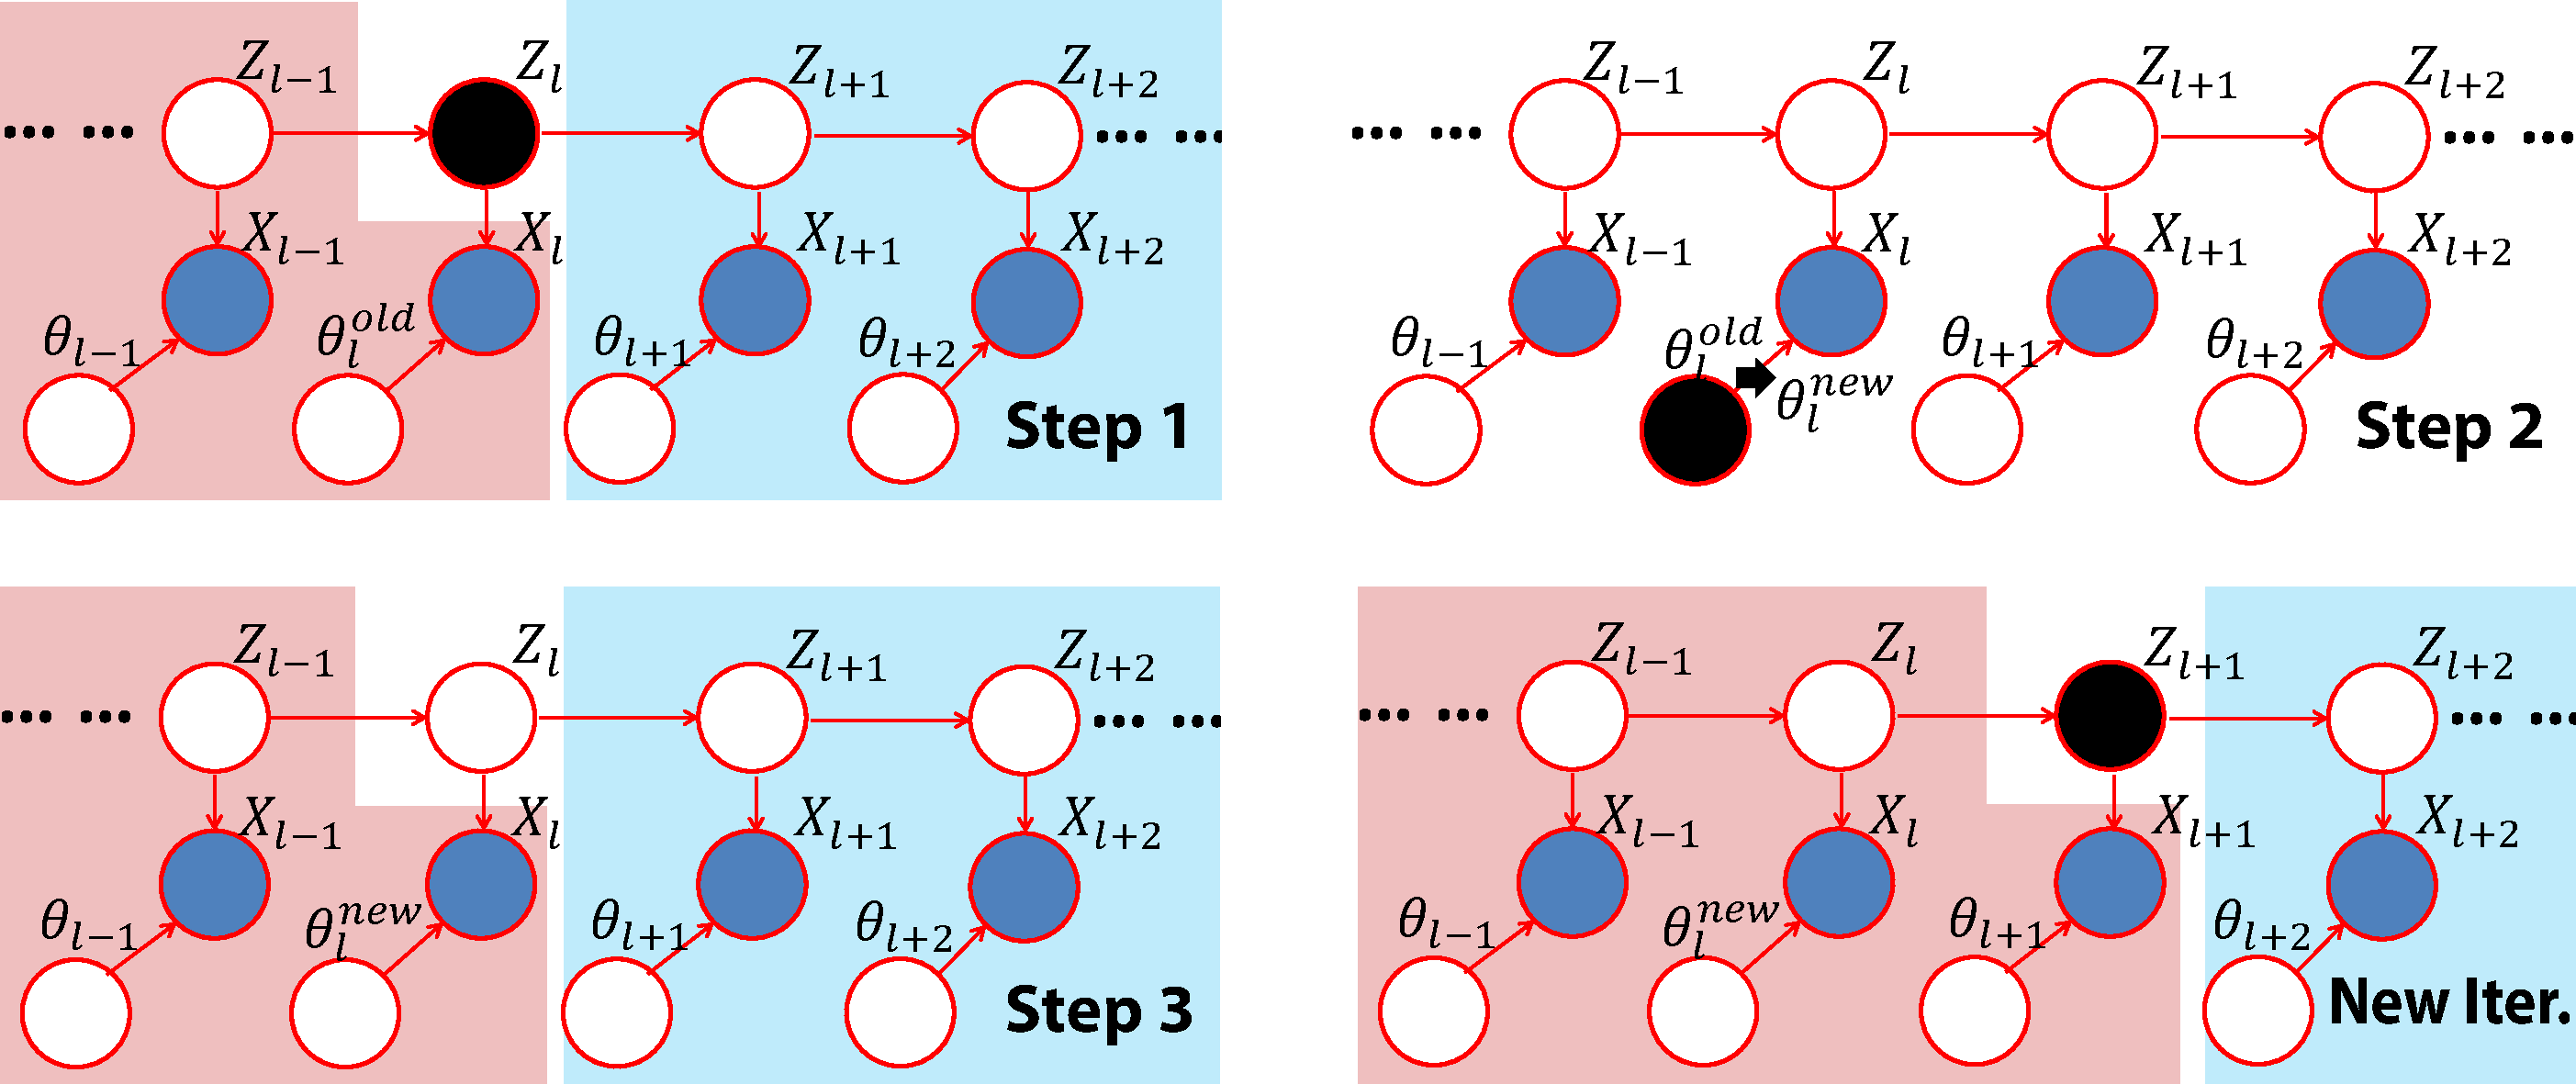
\includegraphics[height=0.42\columnwidth]{chapter3/resource/combine_upschedule.pdf}
\caption{Update schedule. See text for more details.}
\label{fig:updateSchedule}
\end{figure}

The common way to compute approximate distributions is coordinate descent optimization method. Namely, one distribution is optimized while other distributions remain fixed.  Choosing which distribution to optimize over in each step is arbitrary or scheduled based on application, but it always decreases the cost function in Equation (\ref{equ:KLobjective}). %For our multiview stereo depth estimation, we can update all the $q_l(\theta_l)$ first with all $q_m(\bm{Z}^m)$ fixed, and then apply forward-backward algorithm to infer all $q_m(\bm{Z}^m)$ with all $q_l(\theta_l)$ fixed. However
We choose to interleave updates of $q_l(\theta_l)$ and $q_m(\bm{Z}^m)$ as it is able to quickly propagate the correct depth into nearby pixels. For clarity, our explanations below use one chain and omit the image index $m$ for each variable.

For more details on Hidden Markov Chain inference, we refer the reader to text \cite{BishopBook}. The forward-backward algorithm is used to infer the probability of hidden variables $Z_l$.
\begin{equation}
q(Z_l) = \frac{1}{A}\alpha(Z_l)\beta(Z_l),
\label{equ:qZDistribution}
\end{equation}
where A is the normalization factor. $\alpha(Z_l)$ and $\beta(Z_l)$ are the forward and backward message for variable $Z_l$ computed using the following Equations,
\begin{equation}
\alpha(Z_l) = p(X_l|Z_l, \theta_l)\sum_{Z_{l-1}}{\alpha(Z_{l-1})P(Z_l|Z_{l-1})},
\label{equ:forwardMessageUpdate}
\end{equation}
\begin{equation}
\beta(Z_l)=\sum_{Z_{l+1}}\beta(Z_{l+1})P(X_{l+1}|Z_{l+1}, \theta_{l+1})P(Z_{l+1}|Z_{l}).
\label{equ:backwardMessage}
\end{equation}
Both the forward and backward messages are computed recursively (e.g.  $\alpha(Z_l)$ is computed using $\alpha(Z_{l-1})$). In Figure \ref{fig:updateSchedule}, the variables covered in red area and blue area contribute to the forward and backward messages respectively.

We perform the following update schedule as is shown in Figure \ref{fig:updateSchedule}. In step 1, compute $q(Z_l)$ using Equation (\ref{equ:qZDistribution}), (\ref{equ:forwardMessageUpdate}) and (\ref{equ:backwardMessage}) for each source image (\ie $q(Z_l^m)$,$m=1...M$). In step 2, update the depth from $\theta_l^{old}$ to $\theta_l^{new}$ using Equation (\ref{equ:approximateDistTheta2}) or Equation (\ref{equ:approximateDistTheta4}).
%To update depth $\theta_l$, we should compute the selection probability for each of the images, \ie $q(Z_l^m)$,$m=1...M$.
In step 3, with $\theta_l^{new}$, we recompute forward message $\alpha(Z_l)$, which is further used to compute $\alpha(Z_{l+1})$ recursively in Equation (\ref{equ:forwardMessageUpdate}). Next we start at variable $Z_{l+1}$ with the same process until reaching the end of the row in the image. Before the update process, the backward message for each variable can be computed recursively (Equation (\ref{equ:backwardMessage})) and stored in memory.


%%%%%%%%%%%%%%%%%%%%%%%%%%%%%%%%%%%%%%%%%%%%%%%%%%%%%%%%%%%%%%%%%%%%%%%%%%%%%%%%%%%%%%%%%%%
%%%%%%%%%%%%%%%%%%%%%%%%%%%%%%%%%%%%%%%%%%%%%%%%%%%%%%%%%%%%%%%%%%%%%%%%%%%%%%%%%%%%%%%%%%%


\subsection{Algorithm Integration}  \label{sec:algorithm}
%In this subsection, we detail the algorithm given the above formula.
\begin{table}[]
    \small
    \centering
    \begin{tabular}{|l|c|c|}
        \hline
        \multicolumn{3}{|p{13.0cm}|}{{\bf Input}: All images, depthMap (randomly initialized or from previous propagation)}  \\
        \multicolumn{3}{|p{13.0cm}|}{{\bf Output}: Updated depthMap}\\
        \multicolumn{3}{|p{13.0cm}|}{$m$ -- image index, $l$ -- pixel index}\\
        \hline
            & Eq. & Step \\ \cline{2-3}
            {\bf For} $l = L$ to $1$ & &\\
                \hspace{5 mm} {\bf For} $m = 1$ to $M$  & & \\
                    \hspace{10 mm} Compute backward message $\beta_l^m$  &    (\ref{equ:backwardMessage}) &   1 \\
            {\bf For} $l = 1$ to $L$ & &\\
                \hspace{5 mm} {\bf For} $m = 1$ to $M$ & &\\
                  \hspace{10 mm} Compute forward message $\alpha_l^m$  &      (\ref{equ:forwardMessageUpdate}) & 1\\
                  \hspace{10 mm} Compute $q(Z_l^m)$                    &    (\ref{equ:qZDistribution}) & 1\\
                \hspace{5 mm} Draw depth hypotheses by PatchMatch & &\\
                \hspace{5 mm} Estimate $\theta_l^*$ for $q_l(\theta_l)$ &   (\ref{equ:approximateDistTheta2} or \ref{equ:approximateDistTheta4})& 2\\
                \hspace{5 mm} {\bf For} $m = 1$ to $M$  & &\\
                  \hspace{10 mm} Recompute forward message $\alpha_l^m$ & (\ref{equ:forwardMessageUpdate}) & 3\\
        \hline
    \end{tabular}
\caption{The algorithm of a row/column propagation.}
\label{table:algorithm}
\end{table}

We now describe the computational framework implementing our  depth estimation and view selection formulation.
The depthmap is initialized with random values within the depth range. Alternatively, sparse 3D measurements may be included within our initialization. Next, the rightward, downward, leftward and upward propagations are applied in sequence. Each propagation (except in the first iteration) uses the depth results of the former propagation. Within each propagation, updates of the depth and the selection probability are interleaved as described in Section \ref{sec:updateSchedule}. After two or three sweeps, each containing the four direction propagations, the depthmap reaches a stable state.  Convergence may alternatively be verified through tracking the number of modified depth estimates up to a threshold. As each row is independent from other rows given our graphical model and processed in exactly the same way during one propagation, it can be easily parallelized for leveraging GPUs. We describe the algorithm for processing one row within rightward propagation in Table \ref{table:algorithm}.



%\subsection{Refinement}
%\section{Discussion}
{\bf Discussion}.
%We discuss some properties of this algorithm in this section.
The estimation of the exact image-wide MAP for our graphical model would require a Hidden Markov Random Field (MRF) formulation instead of our Hidden Markov Chain approximation.
Our choice of using propagation direction specific chain models was driven by computational efficiency/tractability.
The proposed framework enables us to easily interleave the propagation with hidden variable inference while fostering implementation  parallelism.
The enforcement of smoothness constraints on the hidden variables  enables non-oscillating behavior of our evolving depth estimates.
Our PatchMatch based  framework has linear computational and storage complexity \wrt to input data size while being independent of the size of the depth search space.
Namely, since the number of tested depth hypotheses (3 for each propagation) is small and constant, the computation complexity of our method is $O(W H M)$, where $W$, $H$, and $M$ are the width, height and  number of images.  Methods using complete hypotheses search, e.g. \cite{Sun_ECCV2002_stereoBeliefProp, CombinedDepthOutlier}, require  $O(W H M D)$ computations, where D is the size of hypotheses space
%, which is a tradeoff between computation complexity and precision,
normally reaching up to thousands of hypotheses.
 
 
%%%%%%%%%%%%%%%%%%%%%%%%%%%%%%%%%%%%%%%%%%%%%%%%%%%%%%%%%%%%%%%%%%%%%%%%%%%%%%%%%

%%%%%%%%%%%%%%%%%%%%%%%%%%%%%%%%%%%%%%%%%%%%%%%%%%%%%%%%%%%%%%%%%%%%%%%%%%%%%%%%%
\section{Experiments} \label{sec2:experiment}
We evaluate the accuracy of our method on standard ground truth benchmarks and highlight our robustness on multiple crowd sourced datasets.
In both evaluation scenarios we juxtapose our results with current state-of-the-art methods.
We implemented our method in CUDA and executed on a Nvidia GTX-Titan GPU.
For all experiments, the total number multi-directional propagations is set to 3 and we use  $\sigma = 0.45$ in the likelihood function (Equation (\ref{equ:observationModel})) and $\gamma=0.999$ in the transition probabilities (Equation (\ref{equ:transitionProb})).  %refering to Eqs. \ref{equ:observationModel} and  \ref{equ:transitionProb}, respectively.

\begin{table}[t]
\centering
    \begin{tabular}{|c|c|c|c|c|}
    \hline
         &  2cm &  10cm  & 2 cm & 10cm\\
    \hline
    Error & \multicolumn{2}{|c|}{fountain-P11} & \multicolumn{2}{|c|}{Herzjesu-P9}        \\
    \hline
    Ours & 0.732   & 0.911  & 0.619 & 0.833\\
    \hline
    Ours(P)& 0.769   & 0.929  & 0.650 & 0.844\\
    \hline
    LC \cite{LeastCommitment_3DIMPVT2012} & 0.754 &  {0.930} & 0.649 & 0.848 \\
    \hline
    FUR \cite{FURUKAWA_PAMI2010} & 0.731 & 0.838 & 0.646  & 0.836\\
    \hline
    ZAH \cite{Zaharescu_PAMI2011} & 0.712 & 0.832 & 0.220 & 0.501\\
    \hline
    %TYL &0.732 & 0.822 & \textbf{0.658} & 0.852\\
    TYL \cite{TYL} &0.732 & 0.822 & 0.658 & 0.852\\
    \hline
    JAN \cite{JAN} &0.824 & 0.973 & 0.739 & 0.923\\
    \hline
    \end{tabular}
\caption{The percentage of pixels with absolute error less than 2cm and 10cm. Entries {\em Ours(P)}  and {\em Ours}  denote our results with and without postprocessing.  Reported values are from \citet{LeastCommitment_3DIMPVT2012}.}
\label{tab:data}
\end{table}

%%%%%%%%%%%%%%%%%%%%%%%%%%%%%%%%%%%%%%%%%%%%%%%%%%%%%%%%%%%%%%%%%%%%%%%%%%%%%%%%%%%%%%%%%%%%%%%%%%%%%%%%%%%%%%%%%%%%%%%%%%%%%%%%%%%%%%%%%%
%%%%%%%%%%%%%%%%%%%%%%%%%%%%%%%%%%%%%%%%%%%%%%%%%%%%%%%%%%%%%%%%%%%%%%%%%%%%%%%%%%%%%%%%%%%%%%%%%%%%%%%%%%%%%%%%%%%%%%%%%%%%%%%%%%%%%%%%%%%%%%%%%%%%%%%%%%%%%%%%%
%%%%%%%%%%%%%%%%%%%%%%%%%%%%%%%%%%%%%%%%%%%%%%%%%%%%%%%%%%%%%%%%%%%%%%%%%%%%%%%%%%%%%%%%%%%%%%%%%%%%%%%%%%%%%%%%%%%%%%%%%%%%%%%%%%%%%%%%%%

{\bf Ground truth evaluation}. We evaluated on the Strecha datasets (Fountain-P11 and Herzjesu-P9) presented in \citet{Strecha08}  as  they include ground truth 3D structure measurements.
% In contrast to some stereo methods which need manually select the images around the reference view, we input the entire dataset.
We use all dataset images full resolution, set the  NCC patch size to 15 by 15 and  approximate the depth range from sparse 3D points.
 % give the image resolution of 15x15.
We measure pixel-wise depth errors as our goal is to ge\-ne\-rate a single depthmap instead of one consistent 3D scene model.
We calculate the number of pixels with the depth error less than 2cm and 10cm from the ground truth and compare with \cite{LeastCommitment_3DIMPVT2012, FURUKAWA_PAMI2010, Zaharescu_PAMI2011,TYL,JAN}.
All the pixels with accessible ground truth depth are evaluated to convey both the accuracy and the completeness of the estimated depthmaps.
%The ground truth and the depthmaps of the compared methods are obtained by projecting the 3D meshes on each of the reference cameras.
We omit evaluation of the dataset's two extremal views as done by \citet{LeastCommitment_3DIMPVT2012}.
%The same to \cite{LeastCommitment_3DIMPVT2012}, the two extremal views in the datasets are not included in the evaluation.

We use slanted planes of single orientation instead of fronto-parallel planes.
The single dominant orientation direction can be estimated by projecting sparse 3D points onto the ground plane as described in \citet{Gallup07}.
We further apply two optional depthmap refinement schemes to increase the final accuracy.
Our basic depth refinement uses a smaller NCC patch (5x5), while eliminating random depth sampling, during an additional propagation sweep. We then use deterministic fine-grain sampling (20 hypotheses) in the depth neighborhood ($\pm 1$ cm.) of each  pixel's depth estimate as proposed in \citet{Shen_TIP2013}.
Finally, a median filter of size 9x9 is applied  to each raw depthmap. %We denote the results of our method without and with postprocessing as OM1 and OM2.
Table \ref{tab:data} shows our method is comparable to the state-of-the-art methods. Note the results of \citet{LeastCommitment_3DIMPVT2012, TYL, JAN} are obtained through multi-depthmap fusion, while our method directly estimates  individual depthmaps.

\begin{figure}[]
\centering
\subfloat{
    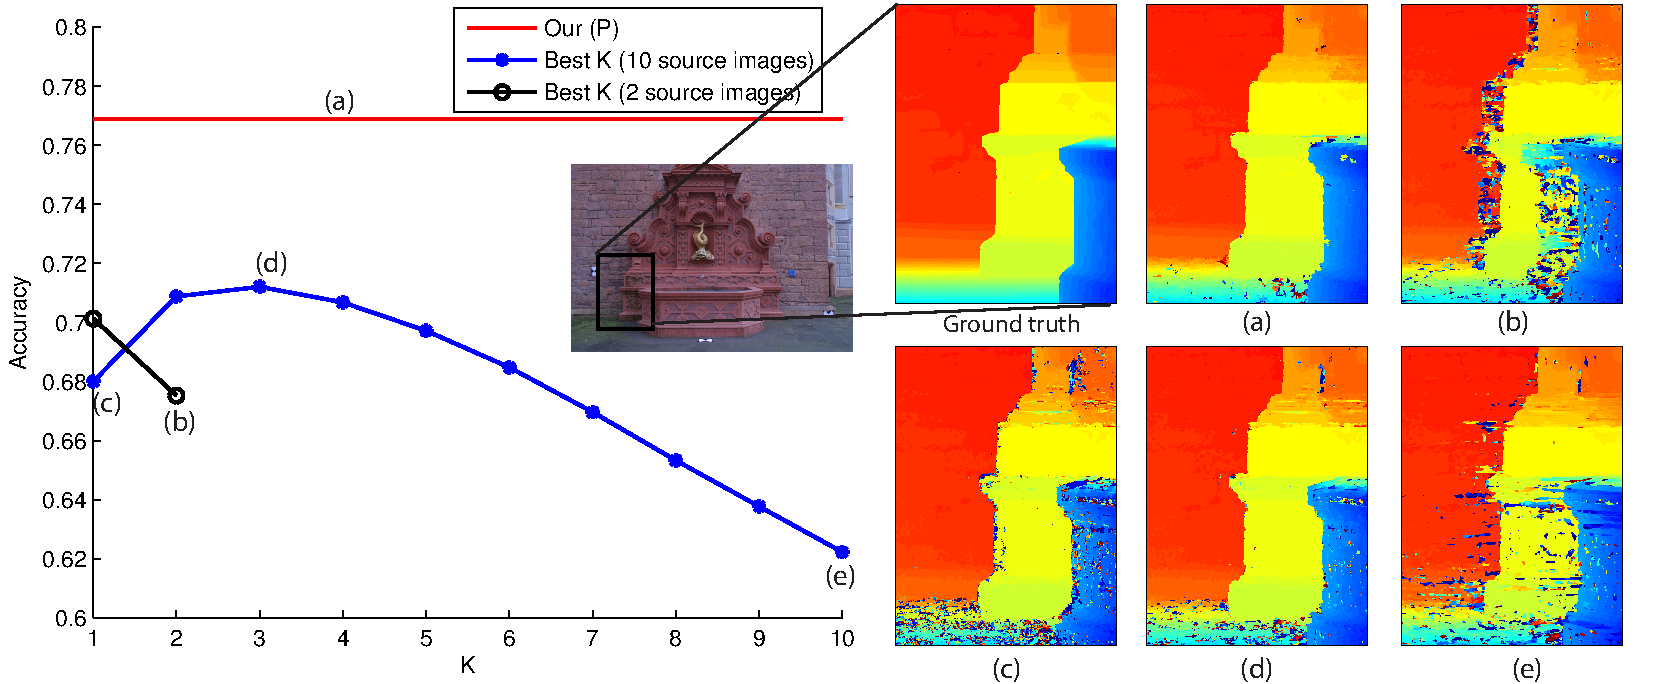
\includegraphics[width=1\columnwidth]{chapter3/resource/subregionCombine.pdf}
}
\caption{Left: Comparison against best-K aggregation. Right: Raw depthmap output of a partially occluded subregion with results for different dataset-aggregation combinations.}
\label{fig:bestK}
\end{figure}

\begin{figure}[]
\centering
\includegraphics[width=0.7\linewidth]{chapter3/resource/planesweepTiming.pdf}
\caption{Fountain dataset performance. Left: Average running time. Right: Percentage of pixels given different thresholds.  PLA is the planesweep algorithm with all source images and K=3, while GOS is the method by \citet{Goesele07}.}
\label{fig:timing}
\end{figure}

{\bf Advantages of pixel level view selection}. Figure \ref{fig:bestK} shows our comparison to the occlusion-robust best-K planesweeping method \cite{handle_occlusion2001}, where
for a given depth hypothesis, the cost is the average of the best K costs, with K being predefined.
When K is set to the number of source images, it degenerates to the basic planesweeping algorithm that computes the cost using all source images.
As opposed to our method with dynamic weights of images used for depth recovery, this method has a worse ability to handle occlusion.
We compute depthmaps of the fountain-P11 data with varying K and otherwise fixed parameters, using 2000 planes.
 %and do the same median filtering afterwards.
The percentage of pixels within 2cm difference from the ground truth is taken as a measure of the error.
We run the planesweeping using two different dataset types. In the first case all 10 source images are used. Alternatively, we use the neighboring left and the right images.
Figure \ref{fig:bestK} shows our results outperform all fixed aggregation schemes and illustrates the raw depthmap output of a partially occluded subregion.



%{\bf Performance and scalability}.
Run times for our method are compared with an optimized GPU planesweeping code.
Figure \ref{fig:timing} shows the linear dependence of computation time to the number of planes as well the diminishing accuracy improvements provided by increasing the search space resolution. Our PatchMatch sampling and propagation scheme only requires depth range specification, foregoing  explicit search space discretization.
 %The number of planes is the tradeoff between depthmap accuracy and computation time.
%As to memory usage, normally the planesweeping needs to store the large cost volume. We conclude that our algorithm beats the planesweeping method in accuracy, speed and memory usage.



{\bf Robustness to noisy SfM estimates}. The  advantage of  pixel-level view selection across the entire dataset is highlighted  in Figure \ref{fig:alexander}, where we compare  our results for corrupted SFM estimates  against those obtained using the approach by \citet{Goesele07}.
%The considered scenario involves a scene with structural symmetry that causes disjoint scene elements  to be incorrectly fused into a single structure.
Figure \ref{fig:alexander} depicts Alexander Nevsky Cathedral in Sofia having indistinguishable structure in the tower structure (\ie view invariant appearance due to structural symmetry). A set of 136 images, comprised by two mutually exclusive subsets observing the front or back, was fed into VisualSFM \cite{WuVSFM} yielding a corrupted 3D model where symmetric structure is fused along with the disjoint camera clusters. The approach by \citet{Goesele07} initially selects a global subset of $~20$ images based  on the corrupted SFM estimates and select  independently for each pixel's depth estimation a fixed number (typically 4) of images from the global subset (similar to using K-best aggregation with K=4). If the global subset is unbalanced or is contaminated by corrupted estimates the completeness of the model is compromised, as shown in Figure \ref{fig:alexander} where the background dome is missing. We consider the entire dataset and implicitly mitigate such outliers. Moreover, we re-executed the code by \citet{Goesele07} with manually filtered camera poses and indeed achieved correct results.

\begin{figure}[]
\centering
\includegraphics[width=1\linewidth]{chapter3/resource/alexander.pdf}
\caption{\label{fig:alexander} Top: Front and back of Alexander Nevsky Cathedral and estimated 3D model. Bottom: original image, depthmap of our method and the method by \citet{Goesele07} with wrong and correct camera poses.
}
\end{figure}

{\bf Robustness to varying capture characteristics}.
\begin{figure*}[]
\centering
\includegraphics[width=1\linewidth]{chapter3/resource/allResultsCombine.pdf}
\caption{Each image triplet  depicts a reference image along with our and Goesele's (\cite{Goesele07}) depthmap output (Best viewed in color).}
\label{fig:ipc}
\end{figure*}
We tested our algorithm on  Internet photo collections (IPC)  downloaded from the Flickr  for six different scenes: Paris Triumphal Arch (195 images), Brandenburg Gate (300 images), Notre Dame de Paris (300 images), Great Buddha (212 images), Mt.~Rushmore (206 images) and Berlin Cathedral (500 images). In order to control GPU memory, we optionally resize imagery to no more than 1024 pixels for each dimension. Camera poses were calculated using VisualSFM \cite{WuVSFM}.
 %These images can have large difference in viewpoints, resolutions, and illuminations. Moreover, scene content can vary drastically due to foreground occlusion.
 %Our algorithm handles datasets containing several hundreds of images without any manual image selection.
The average run time for Berlin Cathedral is 98.3 secs/image.
For illustration, sky region pixels are masked out using the method in \citet{skyDetection} as post-processing.
To compare with the method by \citet{Goesele07}, we run the author's code
\footnote{http://www.gris.informatik.tu-darmstadt.de/projects/multiview-environment/}
on the same dataset with default parameters except for setting the matching window size to the same as ours (7x7). The results shown in Figure \ref{fig:ipc} illustrate that, while both approaches are robust to wide variations in illumination, scale and scene occlusions across the  datasets, our approach tends to provide increased completeness of depthmap estimates. We attribute this to our more flexible view selection framework.  In contrast to the method by \citet{Goesele07}, we avoid making initial hard image discriminations through an initial global image subset.

To quantitatively compare the accuracy of our results with the work by \citet{Goesele07}, in the absence of ground truth geometry for crowd source datasets, we revisit the accuracy of both methods in the Strecha Fountain dataset. The method by \citet{Goesele07} rejects outlier depth estimates based on the NCC values and the viewing angles. Hence, we only compare the accuracy of the reliable pixels as classified by \citet{Goesele07} (comprising  75.4\% of total image pixels).  Figure \ref{fig:compareGoesele} shows our approach outperforming both the method in \citet{Goesele07} and planesweep for high accuracy thresholds. We expect the same accuracy ranking to carry over to the crowd sourced data results.



\begin{figure}[]
\centering
\centering
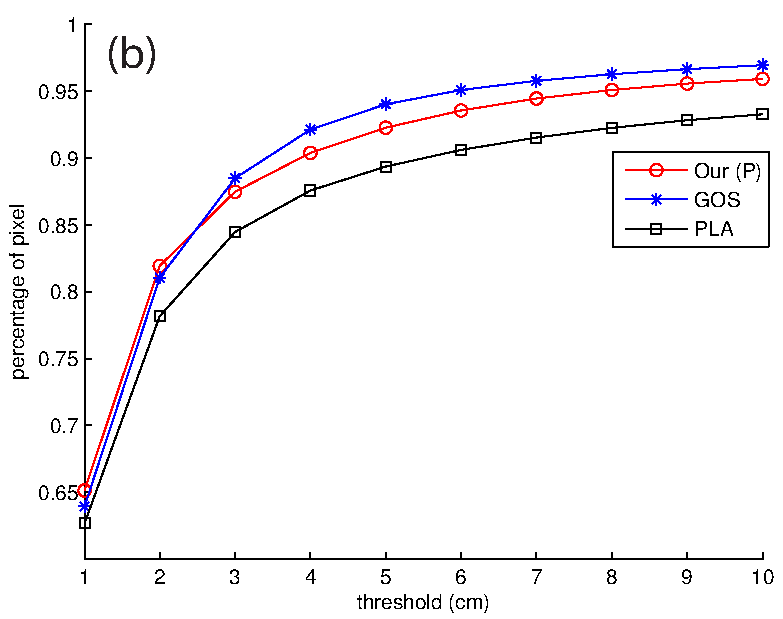
\includegraphics[width=0.60\linewidth]{chapter3/resource/compareGoesele.pdf}
\caption{Fountain dataset performance.Percentage of pixels given different thresholds.  PLA is the planesweep algorithm with all source images and K=3, while GOS is the method by \citet{Goesele07}.}
\label{fig:compareGoesele}
\end{figure}

%%%%%%%%%%%%%%%%%%%%%%%%%%%%%%%%%%%%%%%%%%%%%%%%%%%%%%%%%%%%%%%%%%%%%%%%%%%%%%%%%%%%

%%%%%%%%%%%%%%%%%%%%%%%%%%%%%%%%%%%%%%%%%%%%%%%%%%%%%%%%%%%%%%%%%%%%%%%%%%%%%%%%%%%%
\section{Conclusion}
We have presented an efficient and effective joint solution to the view selection and depth estimation problems in multi-view stereo. Our solution relies on estimating a selection probability of each image in the source image set on the pixel level. The selection probability encodes the existence of contingency issues such as occlusions, specular aberrations and calibration errors. Moreover, by automatically determining reference image data associations with respect to a general source image dataset, we can encompass a larger range input imagery while increasing overall system robustness. Our approach has also extended the PatchMatch algorithms to encompass robust multi-view depth estimation within a probabilistic framework. Reported results achieve state of the art accuracy in ground truth benchmarking while enabling robust operation in crowd sourced datasets. 

%Future research direction include integrating online normal estimation into our approach in order to reduce the reliance on existing sparse data to initialize our plane sweeping direction. We will explore the use of more sophisticated filtering mechanisms as the ones presented in \cite{Hosni12} in order to improve both computational efficiency and estimation accuracy.

%We presented an efficient and effective method for joint view selection and depthmap estimation. Future research direction includes integrating online plane normal estimation for each pixel. We will explore the use of more sophisticated filtering mechanisms such as the one presented in \cite{Hosni12} to further improve both efficiency and accuracy.



%Note more images used does not mean better depthmap accuracy, and it is useful to remove some unrelated images based on camera poses.
%Here we use the entire dataset to show the scalability and robustness of our algorithm.
%Also we found for very few images, using sparse 3D points from SFM to initialize the depthmap helps the algorithm avoiding false local minima.


%For the Strecha's data, we resize the image to 768X512. The NCC patch size is set to 9X9. It takes around 2.5 seconds to generate one depthmap from 10 source images on NVIDIA Geforce 680. For the internet collected data, generating one depthmap of resolutoin 1024X768 from 289 source images with NCC patch size equal to 9X9 takes around 3 minutes. The memory usage is $O(M*W*H)$, where $M$, $W$, $H$ are the number of images, image width, and image height respectively. The memory is mainly used to store images, NCC cost of the current depth, and the backward messages (Eq. (\ref{equ:backwardMessage})). The memory amount can be largely reduced in trade of more computations by recomputing the cost and backward message in each propagation.

%Using more images does not increase the computation time linearly. The computation relies on several factors. If most target images are not useful to recover the depth, then the number of images used for recover the depth for certain pixel will be significantly smaller than $N$. In this case the computation will be smaller, as some images will never be used to test depth of certain pixels. The computation of $S$ scales linearly with the number of images used.

%\begin{figure}[t]
%\centering
%    \includegraphics[height=0.6\columnwidth]{resource/bestK/bestK_error.pdf}
%    \caption{The comparison of our method with best K method. }
%\label{fig:bestK}
%\end{figure}

%\begin{table}[t]
%\centering
%    \begin{tabular}{|p{1.3cm}|p{1.7cm}|p{0.95cm}|p{1.2cm}|p{1.2cm}|}
%    \hline
%        Triumphal Arch &  Brandenburg Gate & Notre Dame& Cathedral & Reichstag\\
%    \hline
%        195 & 290 &  290   & 290 &  290\\
%    \hline
%    \end{tabular}
%\label{table:dataSize}
%\caption{The size of each Internet photo collection datasets}
%\end{table}




\chapter{Joint Object Class Sequencing and Trajectory Triangulation (JOST)} \label{ch:jost}

\section{Introduction}

Techniques of 3D reconstruction from crowd-souced imagery have developped rapidly over the past decades, enabling systems to build 3D models from millions of images \cite{agarwal2011building,Frahm2010,zheng2014patchmatch,Heinly}. 
Despite these advances, the state-of-the-art methods only reconstruct the static part of a scene, but fail on the dynamic part. 
Since dynamic objects are typically the major focus of real-life images, it is of great interest to recover the 3D information of the dynamic objects to enable further applications.

%As the dynamic objects are typically the main focus of imagery, there is an demanding request 
%The main reason is that in typical datasets there is only a single view of any dynamic object, which impedes these methods from valid 3D triangulation.
%Hence, current techniques are not able to determine the 3D position of such objects. 
%This situation is regarded to have a highly limited potential for reconstruction as stated by \citet{Park_ECCV2010} and \citet{Valmadre_CVPR2012}.
In this work, we propose a method to estimate the 3D positions of dynamic objects of the same class moving in a common path from temporally uncorrelated images, \eg~a set of images capturing pedestrians walking on the sidewalk (see Figure \ref{fig:franklin_imgs}). 
The main challenge of the problem resides in the non-current captures of the dynamic objects, which invalidates the traditional 3D triangulation. 
Moreover, each instance of the object is typically observed by only one image and the temporal information across images is unknown. The only constraint available for our problem is the fact that all observed instances of an object class move along a common compact path in the 3D scene, which we define as an object class trajectory. For example, all the pedestrian instances walking on the sidewalk form an object class trajectory.

To attain the object class trajectory, our method simultaneously determines the sequence of the objects along the 3D path and the 3D positions of the objects on the path. Accordingly, this can be deemed as a joint object class equencing and trajectory triangulation, which generalizes the well known sequencing problem \cite{Basha_ECCV2012,Basha_ICCV2013} and the trajectory triangulation problem \cite{Valmadre_CVPR2012,ZhuCL_CVPR11,Park_ECCV2010} into a common framework. We leverage all the observations on different images to recover the object class trajectory, which then gives us the 3D positions of the dynamic objects.

%We formulate our problem as a non-convex optimization problem, and develop a novel solver comprising a step of discrete optimization followed by another step of continuous optimization. 
%The discrete step  a K-partite graph

%In fact, our proposed framework handles both of these problems as special cases. 
%The reconstructed object class trajectory then allows us to solve the generally ill-posed 3D reconstruction of a dynamic object from a single image by constraining the reconstruction on the 3D path of the object class. 
%An example of a single view reconstruction of two pedestrians is shown in Figure \ref{fig:FranklinSingleViewRecon}. %visualizing a generic person at the correct 3D position in the reconstruction of the 3D scene.

\begin{figure}[t]
\centering
\subfloat[]{
\centering
    \includegraphics[height=0.34\linewidth]{chapter4/resource/images_cropped.pdf}
    \label{fig:franklin_imgs}
     \label{fig:franklin_sfm}
    }
\subfloat[]{
\centering
    \includegraphics[height=0.34\linewidth]{chapter4/resource/3DModel.png}
    \label{fig:FranklinSingleViewRecon}
    }
\caption{Left: 3 images of the pedestrian dataset and the output of SFM. Right: The reconstruction of two pedestrians that are captured in the single image. Note we only reconstruction one 3D position for each dynamic object instance. For visualization purposes, a general mesh model is inserted into each estimated position.}
%\end{subfigure}
\label{fig:gmst}
\vspace*{-0.5cm}
\end{figure}

\section{\JOST}

We now detail our method for \jost~from uncontrolled image captures, which in particular removes the constraint of known temporal camera information and known object positions. To perform \jost~from the uncontrolled image set, we proceed as follows
\begin{enumerate}
\item \label{challenges_sfm} Spatially register the cameras to a common 3D coordinate system.
\item \label{challenges_tang} Detect object instances and estimate motion tangents from input imagery.
\item \label{challenges_order} Leverage the image positions of the object instances to simultaneously
\begin{enumerate}
\item Determine a camera ordering compliant with a continuous motion of the objects along a trajectory.
\item Triangulate the geometry of the corresponding motion path.
\end{enumerate}

\end{enumerate}
While we exploit known methods to solve for camera registration, object detection and motion tangents in the images, our main contribution is an algorithm for tackling challenge  \ref{challenges_order}. To tackle this challenge, we model our problem as a non-convex optimization problem, and develop a novel solver comprising a step of discrete optimization followed by another step of continuous optimization. 
Next, we introduce each step in detail.

\subsection{Spatial Registration}
The goal of the initial spatial registration in our method is to establish camera registration in a common coordinate system.
%There exists a large body of possible registration methods in structure from motion that can be used to register the cameras into a common coordinate system.
Given that in all our datasets a fair portion of the images contains static background structure, we use the publicly available structure from motion tool VisualSFM by Wu~\cite{WuVSFM}. It produces the camera registration and the sparse 3D points of the static structure. See Figure \ref{fig:franklin_sfm} for an example.

The obtained camera registration determines the camera center $\mathbf{\tilde{C}}_j$ of the $j$-th camera. In the paper we use bold font letters ${\mathbf x}$ to indicate that an entity is a vector and regular letters $x$ for scalar values. With the known camera calibration and registration, each pixel in the camera defines a ray direction $\mathbf{r}$ in the 3D scene  space. For our object class trajectory, we are only interested in the ray directions $\mathbf r_i$ for the different object $i$  of the desired class (for simplicity we refer in the paper to them as objects) with  $i =1, \dots, N$, where $N$ is the number of detected object class instances  over all frames. Hence, we only aim to compute the ray directions $\mathbf{r}_i$ for pixels belonging to the different detected objects $i$. The ray $\mathbf{X}_i$ in the 3D space represents a 1D subspace on which the imaged object has to lie and is described by:
\begin{equation}
\label{eq:ray}
\mathbf{X}_i(t_i)=\mathbf{C}_i + t_i \cdot \mathbf{r_i},
\end{equation}
where $t_i \geq 0$ is the positive distance from the camera center $\mathbf{C}_i$ along the ray $\mathbf{X}_i$.
In the remaining of the paper, we keep the condition $t_i \geq 0$ implicit for the purpose of concise formulation.
We denote the camera centers as $\mathbf{C}_i$  with $\mathbf{C}_i =\mathbf{\tilde{C}}_j$, where $\mathbf{C}_i$ is the center of the camera $j$ in which the object instance $i$ is detected. Please note that if more than one object is detected in camera $j$, there will be multiple $\mathbf{C}_i$ with identical positions. The unknown true distance of the object instance $i$ along ray $\mathbf{X}_i$ is denoted as $\hat{t}_i$. Once obtained, it determines the 3D object position $\mathbf{\hat{X}}_i$. %Next we turn to detail our object class instance detection and the motion tangent estimation.


\subsection{Object Detection and Motion Tangent Estimation}
\label{sec:detection}
Our proposed joint object class sequencing and trajectory triangulation leverages the motion tangent of the object instances, which is defined as the moving direction of the dynamic object in the 3D space. In this work, both object detection and motion tangent estimation are performed based on a single image.
For trajectory triangulation this has historically been solved by using videos for estimating the motion tangents~\cite{zhao2003face}, but for our proposed \jost~problem, temporal coherence or temporal proximity of the images cannot be assumed. Hence only motion tangent estimation based on a single image is applied.
The particular choice of object and motion tangent estimation method depends on the specific object class and the scenes.
We discuss our particular choices in Section \ref{sec:face_detection}, and for now we assume available the positions on each image defining the rays $\mathbf{X}_i$ and a coarse estimate of the motion tangent $\mathbf{d}_i$ of object $i$.
%quantized every $\theta^{\circ}$ between $-90^{\circ}$ and $90^{\circ}$. 
%In the following 
We determine the 2D position of each detected object $i=1,\dots, N$ on the image by the center of the bounding box.
%i.e. if the object is determined to be present in a connected component of the image, we represent its position through the center of gravity of that region.
%This simplifies the object class trajectories to the trajectory of a single characteristic object point. While in general this has the potential of slightly disturbing the trajectory, we empirically found that does not introduce any significant disturbance.
These object detections provide us a ray $\mathbf{X}_i(t_i)$ for each object observed in a camera, with the ray describing the one-dimensional subspace in which the detected object can be placed in the 3D space.
%Next %we will describe how the rays $\mathbf{X}_i(t_i)$ and the motion tangents of
%the objects are leveraged to compute the object class trajectory.


\subsection{Object Class Trajectory Estimation Problem}
\label{sec:problem}
%piecewise linear represented continuously or discrete
Assuming known rays $\mathbf{X}_i(t_i)$ and the motion tangents $\mathbf{d}_{i}$, we will now define the object class trajectory estimation problem before delving into our data representation and our estimation framework. For the ease of description, we directly leverage the rays $\mathbf{X}_i(t_i)$ of the detected objects $i$ and do not use the camera registration directly as the latter is implicitly present in the ray.

Intuitively, an \oct~describes the motion along a path taken by the observed objects of the desired class through the 3D scene. A path can in general be any continuous curve in the 3D scene space. Since we only have a finite number of observations of objects along the path, we only sample a discrete set of 3D points on the path. The samples along the path are the 3D object positions $\mathbf{\hat{X}}_i$. Here, we represent the path as a combination of  piecewise linear functions in between the sampled object positions $\mathbf{\hat{X}}_i$.
%, but in general any parametric representation of the path can be chosen.
The desired \oct~is the path of minimal length and it can be determined through a minimization of the cost function:
\begin{equation}
\label{eq:pathsimple}
\underset{\mathbf{p}} { \min  }\sum_{(i,j)\in\mathbf{p}}{\|\mathbf{\hat{X}}_i-\mathbf{\hat{X}}_j\|_2^2} \\
\end{equation}
with $\mathbf{p}$ representing the adjacency of the points defining the topology of the path, which is list of adjacency relationships between all the points $\mathbf{\hat{X}}_i$, $i=1, \dots, N$. While the trajectory above is based on the observed 3D object positions $\mathbf{\hat{X}}_i$, we can only observe the rays $\mathbf{X}_i(t_i)$. To determine the \oct, we also need to determine the position of each object $i$ along its viewing ray $\mathbf{X}_i(t_i)$, which defines the 3D position of the object $\mathbf{\hat{X}}_i$.
We propose to find the adjacency relation by optimizing over variables $\mathbf{t}=[ t_1, \dots, t_N ]$ and $\mathbf{p}$ jointly as follows,
%For a set of rays  $\mathbf{X}_i(t_i)$ with $i=1, \dots, N$, the points are determined by the distances $ \mathbf{t}=[ t_1, \dots, t_N ]$. Hence, the optimization from  Equation (\ref{eq:pathsimple}) can be reformulated:
\begin{equation}
\label{eq:pathsimpleray}
\underset{\mathbf{p},\mathbf{t}} { \text{min} }\sum_{(i,j)\in\mathbf{p}}{\|\mathbf{X}_i(t_i)-\mathbf{X}_j(t_j)\|_2^2}. \\
\end{equation}
Given the motion tangents $\mathbf d_i$ estimated from the images, we can further constrain the trajectory, obtaining an optimization problem:
\begin{equation}
\label{equ:costFunc}
\underset{\mathbf{p},\mathbf{t}} { \text{min} }
\sum_{(i,j)\in\mathbf{p}}{\|\mathbf{d}_{i,j}\times(\mathbf{X}_i(t_i)-\mathbf{X}_j(t_j))\|_2^2 + \lambda\|\mathbf{X}_i(t_i)-\mathbf{X}_j(t_j)\|_2^2}, \\
%\nonumber
%\text{with } \mathbf{X_i}=\mathbf{C_i} + t_i \cdot \mathbf{r_i}  ,\quad t_i \geq 0, \quad i =1,2,...N
\end{equation}
where the operator $\times$ is the cross product, $\lambda$ is a positive weight (discussed at length in Sec. \ref{sec:analysis}). The direction $\mathbf{d}_{i,j}$ is selected from $\mathbf{d}_i$ and $\mathbf{d}_j$, as the motion tangent that is closest to the 3D motion direction $\mathbf{X}_i(t_i)-\mathbf{X}_j(t_j)$.
In Eq. (\ref{equ:costFunc}), the penalty of the first term increases if the direction of the vector $\mathbf{X}_i(t_i)-\mathbf{X}_j(t_j)$ deviates from $\mathbf{d}_{i,j}$.
The optimization procedure simultaneously determines both the adjacency $\mathbf{p}$ of the rays and the positions of the objects through $\mathbf{t}$.

Traditionally, these problems have been treated separately as either a sequencing problem,
%\en{add a couple of references. Jan, I do not know about this. we can discuss tomorrow. There are actually works  \cite{Basha_ECCV2012}and \cite{Basha_ICCV2013} doing image sequencing. But those paper does not have 3D points available. I think given dynamic 3D points, doing the sequencing is trivial.}
where the 3D points are given and only the sequence of traversal needs to be estimated, or as a trajectory triangulation problem \cite{Park_ECCV2010,Valmadre_CVPR2012}, where the sequence of observations for the trajectory is given and the 3D points along the trajectory need to be determined. Our proposed method generalizes these problems into a common framework to allow the simultaneous estimation of the adjacency of observations and the 3D position of the observations. %After defining the cost function (Eq. (\ref{equ:costFunc})) for the optimization problem to determine the object class trajectory,
Optimization of the non-convex function in Eq.~(\ref{equ:costFunc}) is inherently difficult. To achieve this, we propose a new discrete-continuous  optimization strategy through the Generalized Minimum Spanning Tree (GMST).

\subsection{Generalized Trajectory Graph}
\begin{figure}[t]
\centering
    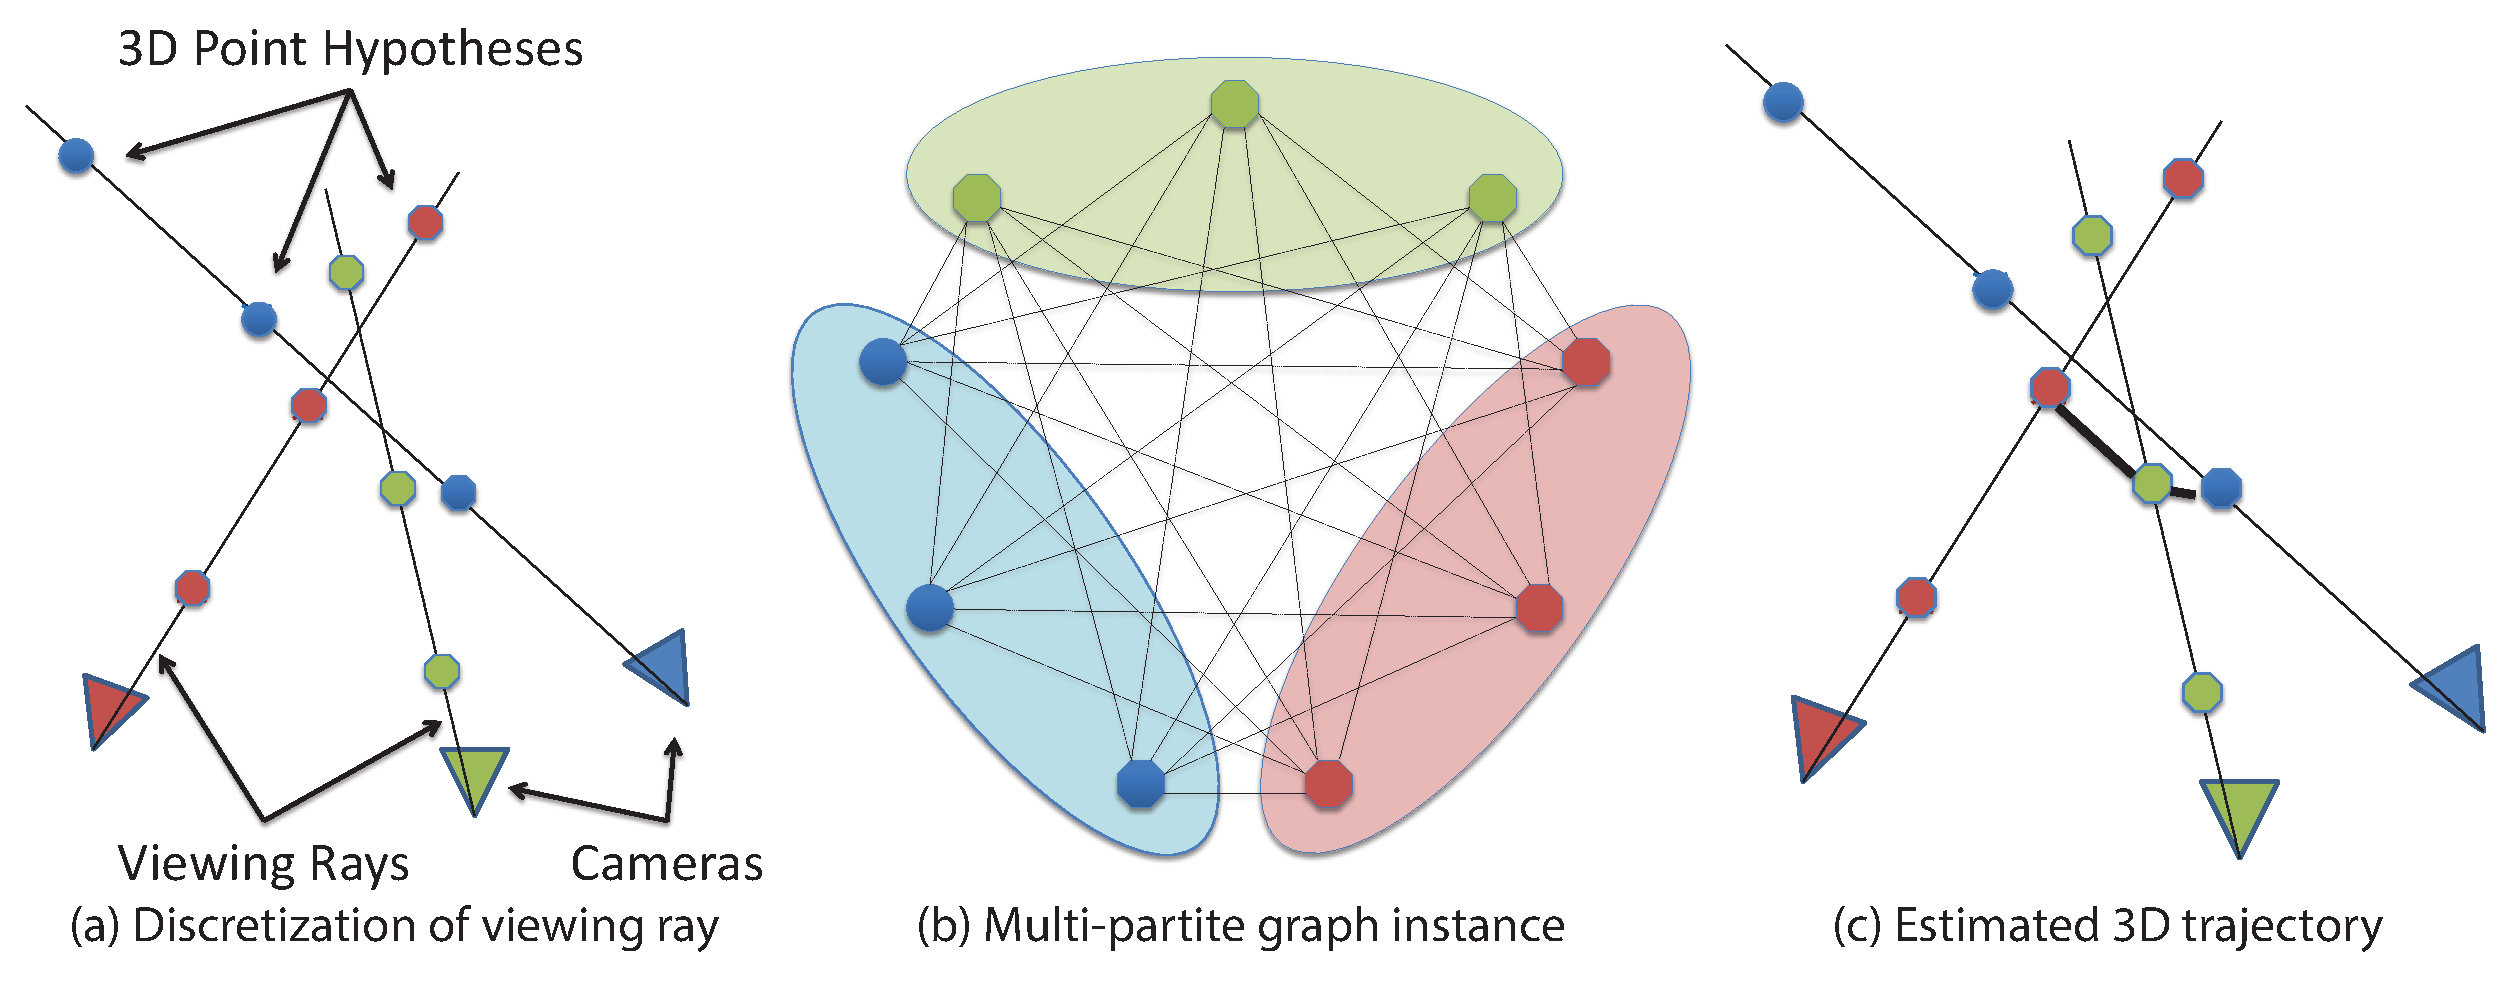
\includegraphics[width=1\columnwidth]{chapter4/resource/gmst_eccv.pdf}
\caption{Illustration of GMST. See the text for more details.}
%\end{subfigure}
\label{fig:gmst}
\end{figure}

\label{sec:gmst}
To determine the \oct, we conceptually have to choose for each ray $\mathbf{X}_i(t_i) $ the 3D point, and simultaneously determine the adjacency $\mathbf{p}$ representing the adjacency relations of the rays $\mathbf{X}_i(t_i) $, which defines the topology of the \oct.
Our discrete-continuous optimization strategy first uses a Generalized Minimum Spanning Tree (GMST) to find adjacency $\mathbf{p}$, and followed by a convex optimization over $\mathbf{t}$ with $\mathbf{p}$ being fixed.

In the discrete optimization step, we map the continuous problem of finding the 3D point along each ray to a discrete problem of selecting a 3D point out of a set of discrete 3D points. Then we determine one 3D point along each ray and the adjacency $\mathbf{p}$ by computing the GMST on an undirected multipartite graph $\cal{G}(V,E)$~\cite{MyungLT_95}. This allows us to simultaneously  determine the topology and the discrete 3D object positions.

An undirected multipartite graph is a graph whose vertices are partitioned into $N$ partite sets $\left\{V_1, \dots, V_N\right\}$ with $\vert V_i \vert = k$, while fulfilling ${\cal V}=V_1 \cup V_2 \cup \dots \cup V_N$ and $V_o \cap V_p = \emptyset, \forall o\neq p$, with $o,p \in \{1, \dots, N \}$. The multipartite graph $\cal{G}(V,E)$ has only edges between the different partite sets  of vertices $V_o$, and all edge cost are non-negative. Now we will detail on how we define the graph $\cal{G}(V,E)$ based on Eq.~\ref{equ:costFunc}.

Each ray $\mathbf{X}_i(t)$ defines a one dimensional constraint on the 3D position of the object. We discretize the ray to obtain a discrete set of potential depth estimates. This leads to a finite set of possible 3D positions along the ray (see Figure \ref{fig:gmst}(a) for an illustration), defining a finite set of 3D point hypotheses %$\mathbf{\hat{X}}_i^o=\mathbf{X}_i (\hat{t}_o)$ with $\vert t_o \vert = k$,
$\{\mathbf{\hat{X}}_i^o|o=1,\dots,k \}$,
where $k$ is the number of the discrete hypotheses along the ray.
In our representation, each 3D point $\mathbf{\hat{X}}_i^o$ establishes node $V_i^o$ in the graph. The set of nodes $\{V_i^o|o=1, \dots, k\}$ related to the ray $\mathbf{X}_i(t)$ of object $i$ defines a partite set of nodes $V_i$ in the graph $\cal{G}(V,E)$. 
Given that no nodes within a group have any connecting edges, it enforces the traversal of the graph to be constrained among partite sets. 
%This is  consistent with the understanding of moving the different instances of an object class in the scene to determine the object class trajectory.

We now define the edge cost of the multipartite graph based on Eq. (\ref{equ:costFunc}).
The multipartite graph only has edges between the nodes from different partite sets.
%Given the properties of the multipartite graph we only insert edges between the nodes that are in different partite sets of nodes.
We define the edge direction $\mathbf{d}_{i,j}$ between any two nodes $V_i^o$ and $V_j^p$ in the partite set $i$ and partite set $j$ respectively, as the consistency of the 3D motion with the motion tangents $\mathbf d_i$ and $\mathbf d_j$ (see Sec. \ref{sec:detection}). This definition comes from the intuition that the edge direction should be compliant with the motion tangent observed in the images. Given the motion of two objects $i$ and $j$ and their respective motion tangents $\mathbf d_i$ and $\mathbf d_j$, it is clear that the motion between the points $\mathbf{X}_i^o$ and $\mathbf{X}_j^p$ (associated with the nodes $V_i^o$ and $V_j^p$) should be close in direction to at least one of the motion tangents $\mathbf d_i$ and $\mathbf d_j$.
%Then one can think that the edge direction $\mathbf{d}_{i,j}$ should be either $\mathbf{d}_i$ or $\mathbf{d}_j$, as is shown in Figure \ref{fig:node_DirectionA}. Any edge parallel to $\mathbf{d}_i$ or $\mathbf{d}_j$ should be encouraged.
Therefore, we define the edge cost $e(V_i^o,V_j^p)$ of the edge between the nodes $V_i^o$ and $V_j^p$ as

\begin{equation}
\label{eq:edgecost}
e(V_i^o,V_j^p)=\text{min}(\|\mathbf{d}_i\times(\mathbf{X}_i^{o}-\mathbf{X}_j^{p})\|_2^2, \|\mathbf{d}_j\times(\mathbf{X}_i^{o}-\mathbf{X}_j^{p})\|_2^2) +\lambda\|\mathbf{X}_i^{o}-\mathbf{X}_j^{p}\|_2^2.
\end{equation}
If only considering the first term in Eq. (\ref{eq:edgecost}), edges with 3D motion directions that are approximately parallel to $\mathbf{d}_i$ or $\mathbf{d}_j$ have lower  cost than those are at an angle to both $\mathbf{d}_i$ and $\mathbf{d}_j$. For instance, %for the edge cost from Eq. (\ref{eq:edgecost}),
Edge 1 and Edge 3 in Figure \ref{fig:node_DirectionB} have a relatively lower cost than Edge 2 because Edge 1 is parallel to $\mathbf{d}_j$ and Edge 3 is parallel to $\mathbf{d}_i$.

\subsection{GMST}
\begin{figure}[t]
\centering
\subfloat[]{
    \includegraphics[height=0.19\textheight]{chapter4/resource/nodeDirection1_cropped.pdf}
    \label{fig:node_DirectionA}
}
\subfloat[]{
    \includegraphics[height=0.19\textheight]{chapter4/resource/nodeDirection2_cropped.pdf}
    \label{fig:node_DirectionB}
}
\subfloat[]{
    \includegraphics[height=0.19\textheight]{chapter4/resource/edgeReduction_cropped.pdf}
    \label{fig:node_edgeRemove}
}

\caption{In Figure \ref{fig:node_DirectionA}, the black nodes shows the real positions of dynamic objects. The red vector represents the direction associated with each object. In the shown example, $\mathbf{d}_{i,j}$ equals $\mathbf{d}_{i}$.  }
%\end{subfigure}
\label{fig:nodeDirection}
\end{figure}

A Generalized Minimum Spanning Tree (GMST) on the graph $\cal{G}(V,E)$ is a tree of minimal cost that spans \emph{exactly one node} from each partite set $V_i$. GMST problem degenerates to a typical minimum spanning tree problem \cite{Cormen:2001:IA:580470} if each of the partite sets contains only one node.
For our proposed graph, it means a GMST includes exactly one 3D point from each ray. Furthermore, GMST prefers the edge $e(V_i^o,V_j^p)$ that has small value of $\|\mathbf{X}_i^o-\mathbf{X}_j^p\|^2$ and is compliant with the motion tangents in the images, as those edges have lower edge cost. Accordingly, a GMST is our desired solution for estimating the \oct. Notice that if we sample infinite number of 3d points along each viewing ray, the corresponding GMST problem is equivalent to the original cost function Eq. (\ref{equ:costFunc}).% before discretization for the multipartite graph formulation.

The multipartite graph defined above contains a large amount of edges, which increases the complexity of computing the GMST.
We use a deterministic way introduced by Ferreira et al. \cite{Ferreira_ESWA2012} to remove those edges that are guaranteed not to be included in the GMST. Here we use a specific toy example in Figure \ref{fig:node_edgeRemove} to illustrate the method. If the cost of edge $(u,v)$ is larger than any cost of the 6 edges $(u,n_l)$ and $(v,n_l)$, $l=1,2,3$, the edge $(u,v)$ is safe to be removed. A simple proof is that if edge $(u,v)$ exists in the computed GMST, we could remove edge $(u,v)$ and replace it by one of the 6 edges to obtain a new GMST with lower cost. Therefore, edge $(u,v)$ can not be present in the GMST. Moreover, it is plausible to explore other ways to remove edges based on given prior information. For instance, if it is known the pairwise neighboring 3D objects are close in 3D space, we can safely remove the edges that connects two farther point hypotheses by applying a threshold.

The GMST problem was first introduced by Myung \citet{MyungLT_95} and was extensively studied in the past two decades \cite{Feremans_LL02,MyungLT_95,Oncan_CL08,Ferreira_ESWA2012,Dror_EJOR} due to its wide applications in  telecommunications, agriculture watering, and facility distribution design \cite{MyungLT_95,Dror_EJOR}. Unlike the minimum spanning tree (MST) problem, which can be solved in polynomial time, finding the GMST is proved to be NP-hard \cite{MyungLT_95}. Myung \etal \cite{MyungLT_95} and Feremans \etal \cite{Feremans_LL02} propose several integer programming formulations for the GMST problem. However, those provide no guarantee of efficiency, especially when the problem scale is large. The computational challenge of the GMST problem has led to the development of metaheuristics \cite{Oncan_CL08,Ferreira_ESWA2012} that search the hypothesis space, and are empirically shown to be effective.

We exploit the state-of-the-art GRASP-based approach proposed by Ferreira \etal \cite{Ferreira_ESWA2012}. GRASP (Greedy Randomized Adaptive Search Procedure) is a metaheuristic that consists of iterations made up two phases: 1) solution construction and 2) solution improvement through local search. \citet{Ferreira_ESWA2012} proposed the method considering several solution construction algorithms, a local search procedure, and two additional mechanisms: path-relinking and iterative local search. We refer readers to their paper \cite{Ferreira_ESWA2012} for more details.

The output of GMST computation is the estimation of the 3D points $\mathbf{\widehat{X}}$ and the adjacency topology of the \oct. Then $\mathbf{d}_{i,j}$ equals one of $\mathbf{d}_i$ and $\mathbf{d}_j$  that has smaller angle to the vector $\mathbf{\widehat{X}}_i - \mathbf{\widehat{X}}_j$,
\begin{equation}
\mathbf{d}_{i,j}= \underset{\mathbf{d}\in{\{\mathbf{d}_i, \mathbf{d}_j}\} }{\arg\!\max}(|\mathbf{d} \cdot (\mathbf{\widehat{X}}_i - \mathbf{\widehat{X}}_j)| ).
%\mathbf{d_{i,j}} = \text
\end{equation}
%The solution described by the GMST provides us with the discretized 3D points $\mathbf{X}_i^{o}$ as the nodes of the GMST and with the adjacency $\mathbf{p}$ of nodes as defined by the GMST. This represents the rays of the objects as a discrete \oct. While the adjacency is naturally a discrete entity the 3D points of the object along the motion path are naturally continuous entities. Hence, we accept
We fix the adjacency $\mathbf{p}$ given by the GMST, and add a final continuous refinement step for the 3D object position $\mathbf{\hat{X}}_i$, through a convex program optimization over variable $\mathbf{t}$
%To achieve this we fix the adjacency $p$ and only optimize over the object positions $\mathbf{t}$ in Equation (\ref{equ:costFunc}). This leads to the following optimization problem:
\begin{equation}
\underset{\mathbf{t}} { \text{min} }
\sum_{(i,j)\in{\mathbf{p}}}{\|\mathbf{d}_{i,j}\times(\mathbf{X}_i-\mathbf{X}_j)\|_2^2 + \lambda\|\mathbf{X}_i-\mathbf{X}_j\|_2^2}
\label{equ:costFunc_continuous}
\end{equation}
%Solving the convex program in Equation (\ref{equ:costFunc_continuous}) provides the continuous solution for the 3D object positions along the \oct.


\subsection{Reconstructability Analysis} \label{sec:analysis}

Now we analyze the reconstructability of the proposed method, i. e. determining under which conditions the solution of Eq. (\ref{equ:costFunc}) generates accurate 3D points. The direct analysis of Eq (\ref{equ:costFunc}) is difficult, as it needs to determine in which situation the adjacency $\mathbf{p}$ with minimum cost, out of $N^{N-2}$ possible adjacencies (\cite{wiki_cayley_alg}), corresponds to the \oct. %This requires us to relates the camera centers and real 3D object positions.
We find that having the motion tangent constraint reduces the possibility of finding the wrong adjacency $\mathbf{p}$. Hence, we focus on  the reconstructability of the continuous method Eq. (\ref{equ:costFunc_continuous}) given the adjacency $\mathbf{p}$.

Assume we already know the ground truth 3D point $\mathbf{{X}}_i^*$ of object $i$, $i=1,\dots,N$. Given that $\mathbf{{X}}_i^*$ is present on the viewing ray $\mathbf{X}_i$, we move the camera center $\mathbf{C}_i$ to $\mathbf{X}_i^*$ along the ray $\mathbf{X}_i(t)$ in direction $\mathbf{r}_i$. Then any point on the line that passes through $\mathbf{X}_i^*$ and has ray direction $\mathbf{r}_i$ can be represented as $\mathbf{X}_i (s_i)= \mathbf{X}_i^* + s_i \cdot \mathbf{r}_i$, where $s_i$ is the signed distance (not the positive distance as defined by the $t_i$). Then Eq. (\ref{equ:costFunc_continuous}) can be reformulated as:
\begin{equation}
\label{equ:costFunc_analysis}
\underset{\mathbf{s}} { \text{min} }
\sum_{(i,j)\in{\mathbf{p}}}{\|\mathbf{d}_{i,j}\times(\mathbf{X}_i(s_i)-\mathbf{X}_j(s_j))\|_2^2 + \lambda\|\mathbf{X}_i(s_i)-\mathbf{X}_j(s_j)\|_2^2}, \\
\end{equation}
where $\mathbf{s}=[s_1, \dots, s_N]$. Though $s_i$ is signed distance and $t_i$ is positive distance, minimizing Eq. (\ref{equ:costFunc_continuous}) and Eq. (\ref{equ:costFunc_analysis}) still output the same 3D point positions, as long as the computed 3D points in Eq. (\ref{equ:costFunc_analysis}) are in front of the camera centers. We will see that this is normally true, because the computed 3D points are typically close to their ground truth position if the system is well-conditioned.

We denote the solution of Eq. (\ref{equ:costFunc_analysis}) as $\mathbf{s}^\text{opt}$. The true 3D points are ideally reconstructed if $\mathbf{s}^\text{opt}=0$, since $\mathbf{X}_i(0)$ equals to $\mathbf{{X}}_i^*$ given $\mathbf{s}^\text{opt}=0$.
More specifically, $\mathbf{s}^\text{opt}$ equals the signed Euclidean distance between the 3D points produced by Eq. (\ref{equ:costFunc_continuous}) and the ground truth $X_i^*$.
Therefore, $\|\mathbf{s}^\text{opt}\|$ is the error of the estimated 3D points by Eq. \ref{equ:costFunc_continuous}.
In the remaining of this section, we further analyze when $\|\mathbf{s}^\text{opt}\|$ is small to understand the quality of the estimated 3D points. %achieved approximation.

The minimum value of Eq. (\ref{equ:costFunc_analysis}) is achieved at the point where the first derivative relative to $\mathbf{s}$ equals 0. This produces a linear equation system $\mathbf{A}\mathbf{s}^\text{opt}= \mathbf{b}$, where the $i$th row and $j$th column of matrix $\mathbf{A}$ is
\begin{equation}
A_{ij}= \begin{cases}
%\mathbf{r}_i\cdot\mathbf{r}_j, & \text{if } (i,j)\in T \text{ and } i\neq j \\
\lbrack(\mathbf{r}_i\cdot\mathbf{d}_{i,j})\mathbf{d}_{i,j}-(1+\lambda)\mathbf{r}_i\rbrack\cdot\mathbf{r}_j  & \text{if } i\neq j \text{ and } (i,j)\in \mathbf{p}\\
0, & \text{if } i\neq j \text{ and } (i,j)\notin \mathbf{p}\\
\sum_{(i,k)\in{\mathbf{p}}}{\lbrack 1+\lambda - (\mathbf{r}_i\cdot\mathbf{d}_{i,k})^2 \rbrack } & \text{if } i=j
\end{cases}
\label{equ:A}
\end{equation}
The $i$th element of vector $\mathbf{b}$ is
\begin{equation}
b_i=\sum\nolimits_{(i,k)\in{\mathbf{p}}}(\mathbf{X}_k^*-\mathbf{X}_i^*)\cdot \lbrack(1+\lambda)\mathbf{r}_i - (\mathbf{r}_i\cdot \mathbf{d}_{i,k})\mathbf{d}_{i,k} \rbrack
\label{equ:b}
\end{equation}
Eq. (\ref{equ:A}) and Eq. (\ref{equ:b}) have the following interesting properties:
\begin{enumerate}
\item If $\mathbf{b}$ is 0, $\mathbf{s}^\text{opt}$ equals 0, which means the solution of Eq. (\ref{equ:costFunc_continuous}) recovers the true 3D points. There are a few situations  $\mathbf{b}$ equal 0. (1) In the case of a static object $\mathbf{X}_i^* = \mathbf{X}_k^*$, $\mathbf{b}$ equals 0 based on Eq. (\ref{equ:b}). (2) Careful observation reveals that if $\lambda$ is set to $0$, in Eq. (\ref{equ:b}) the vector $(1+\lambda)\mathbf{r}_i - (\mathbf{d}_{i,k}\cdot \mathbf{r}_i)\mathbf{d}_{i,k}$ is perpendicular to vector $\mathbf{X}_i^*-\mathbf{X}_k^*$ (Figure \ref{fig:b_lambda0}), hence $b_i=0$. However, we will show that with $\lambda=0$, the linear system $\mathbf{A}\mathbf{s}= \mathbf{b}$ is unstable due to the high condition number of $\mathbf{A}$. (3) As shown in Figure \ref{fig:b_lambdaBiggerthan0}, as $\lambda$ increases from 0, the two vectors slowly deviate from being perpendicular. Therefore, $b_i$ is likely to be small if $\lambda$ is close to 0.
\item Since we can not control 3D positions and there are typically small measurement errors in $\mathbf{d}_{ij}$, $\mathbf{b}$ does not exactly equal to 0. This can be regarded as a small disturbance of $\mathbf{b}$ around $\mathbf{0}$. For the linear system $\mathbf{A}\mathbf{s}^\text{opt}= \mathbf{b}$, one can think of the condition number $\kappa(\mathbf A)$ as being (roughly) the rate at which the solution, $\mathbf{s}^{\text{opt}}$, will change with respect to a change in $\mathbf{b}$. $\kappa(\mathbf A)$ is available as it solely depends on $\mathbf{r}_i$, $\mathbf{d}_{i,j}$ and $\lambda$, but not on the ground truth 3D points $\mathbf{X}^*$. Therefore, we can roughly estimate the reliability of the reconstructed 3D points by computing $\kappa(\mathbf A)$. Moreover, we empirically found that the condition number of matrix $\mathbf{A}$ is inversely related to $\lambda$. The condition number shown in Figure \ref{fig:conditionNum_lamda} is computed using 100 random cameras, and averaged over 200 trials. We can see $\kappa(\mathbf A)$ is large if $\lambda$ is close to 0 and drop dramatically with small $\lambda$. Then $\kappa(\mathbf A)$ decreases monotonically and slowly as $\lambda$ increases. In our experiments, we choose $\lambda=\frac{1}{15}$ as a balance of having good chance of small $\mathbf{b}$ and the stability of the linear system.
\end{enumerate}
In conclusion, if the adjacency $\mathbf{p}$ is correctly found, the reconstructabililty of the object class trajectory mainly depends on the condition number of the linear system. Given the well-conditioned system and correct motion tangent $\mathbf{d}_{i,j}$, we are able to reconstruct the 3D positions close to the ground truth.

\begin{figure}[t]
\centering
%\begin{subfigure}[b]{0.3\textwidth}
\subfloat[$\lambda=0$]{
    \includegraphics[height=0.17\textheight]{chapter4/resource/analysis_1_cropped.pdf}
    \label{fig:b_lambda0}
}
\subfloat[$\lambda>0$]{
    \includegraphics[height=0.17\textheight]{chapter4/resource/analysis_2_cropped.pdf}
    \label{fig:b_lambdaBiggerthan0}
}
\subfloat[$\kappa(\mathbf{A})$ versus $\lambda$]{
    \includegraphics[height=0.17\textheight]{chapter4/resource/conditionNum_lamda.pdf}
    \label{fig:conditionNum_lamda}
}
\caption{Left two: Plot of Eq. (\ref{equ:b}) with $\lambda=0$ and $\lambda>0$. Right: $\kappa(\mathbf{A})$ given different $\lambda$.}
\label{fig:b}
\end{figure}

%%%%%%%%%%%%%%%%%%%%%%%%%%%%%%%%%%%%%%%%%%%%%%%%%%%%%%%%%%%%%%%%%%%%%%%%%%%%%%%%%%%%%%%%%%%%%%%%%%%

%%%%%%%%%%%%%%%%%%%%%%%%%%%%%%%%%%%%%%%%%%%%%%%%%%%%%%%%%%%%%%%%%%%%%%%%%%%%%%%%%%%%%%%%%%%%%%%%%%%
\section{Object Detector and Motion Tangent Estimation}
\label{sec:face_detection}
Before presenting our experimental evaluation, we first briefly describe the particular object detectors we use in our experiments.
Single image based object detection is a well studied problem in computer vision with a wide variety of method readily available~\cite{Zhang2006Local,Dalal2005HOG,lsvm-pami}. Similarly, there is a large number of motion tangent estimation methods in the literature~\cite{Blanz2003face,Gu20063D,jain2010fddb,jones2003fast}.
%While a combination of those methods would yield the desired detections and motion tangents,
We opt for leveraging the method that jointly determines the face position and its motion tangent direction~\cite{Xiangxin_CVPR12}.
%We applied the unified method proposed by Xiangxin \etal \cite{Xiangxin_CVPR12} to jointly detect pedestrian faces and estimate their corresponding motion tangents.
%The method  models the faces as mixtures of tree structures based on shared facial landmarks. 
In our experiments,
%a single template is shared for all 99 facial landmark parts across all 13 mixtures.
the detection threshold is set to $-0.35$ to avoid false detections, as the false alarm may disturb our algorithm. Our chosen detectors provide a motion tangent of object $i$ that is  quantized every $\theta=15^{\circ}$ in the range of $-90^{\circ}$ and $90^{\circ}$.

%To further improve the detection of pedestrians at larger distances we default to a deformable parts
For cars and pedestrians with small faces in the image, we default to the deformable parts
detector~\cite{lsvm-pami,voc-release5}. %, which could also be used for the detection of cars. %This detector utilizes HOG features.
We used the pre-trained model with detection threshold $0.35$.
%The deformable part-based models are discriminatively learned using latent SVMs.
%We used the pre-trained pedestrian model from the INRIA person dataset~\cite{Dalal2005HOG} with detection threshold $0.35$.
% and the \en{ do we have a car experiment? If not we need to take the car out here} car model from the PASCAL dataset~\cite{pascal-voc-2010} with detection threshold $0.1$.
%We again chose higher detection thresholds to avoid false positives. Next we will describe the experimental evaluation of our \jost.
The moving directions of the pedestrians and cars are estimated using the 3D point cloud (output of VisualSFM) of the background wall by assuming the dynamic objects move parallel to the wall. This is normally true for the Manhattan Scene. Some of the detection results are shown in Figure \ref{fig:detection}.
%\begin{figure}[t]
%\centering
%\subfigure[Face detection]{
%\subfigure{
%    \includegraphics[width=0.4\textwidth]{resource/detection/face_detection.png}
%    \label{fig:face_detection}
%    }
%\quad
%\subfigure[Pedestrian detection]{
%\subfigure{
%    \includegraphics[width=0.4\textwidth]{resource/detection/ped_detection.png}
%    \label{fig:pedestrian_detection}
%    }
%\caption{Detected objects and estimated motion tangents using different detectors.}
%\label{fig:detection}
%\end{figure}

\begin{figure}[t]
\centering
\begin{tabular}{c c c}
\includegraphics[width=0.3\textwidth]{chapter4/resource/ped_seq_3.png} & \includegraphics[width=0.3\textwidth]{chapter4/resource/IMG_3375.png} &
\includegraphics[width=0.3\textwidth]{chapter4/resource/IMG_3000-alldect.png}  \\
\includegraphics[width=0.3\textwidth]{chapter4/resource/ped_seq_4.png} &
\includegraphics[width=0.3\textwidth]{chapter4/resource/IMG_3365.png} &
\includegraphics[width=0.3\textwidth]{chapter4/resource/IMG_3073-alldect.png}
\end{tabular}
\caption{Detected objects and estimated motion tangents using different detectors.}
\label{fig:detection}
\end{figure}


%%%%%%%%%%%%%%%%%%%%%%%%%%%%%%%%%%%%%%%%%%%%%%%%%%%%%%%%%%%%%%%%%%%%%%%%%%%%%%%%%%%%%%%%%%%%%

%%%%%%%%%%%%%%%%%%%%%%%%%%%%%%%%%%%%%%%%%%%%%%%%%%%%%%%%%%%%%%%%%%%%%%%%%%%%%%%%%%%%%%%%%%%%%
\section{Experiments}
We evaluate our algorithm on both synthetic and real datasets.
The GMST algorithm used in our method \cite{Ferreira_ESWA2012} searches the hypothesis space, which stops either the GMST cost is under a preset value or the run time reaches a preset limit. For all experiments, we use the time limit to stop searching, given the lack of an adequate {\em a priori} approximation of the true  GMST cost for each dataset.
\begin{table} [b]
\centering
\begin{tabular}{|c|c|c|c|c|c|c|}  \hline
               & single line & T junction & double lines & half circle & sine wave & cross \\
  \hline
  $\text{error}_A$ & 0.5963 & 1.9688 & 1.5169 & 2.3751  & 2.3705 & 3.4111\\
  \hline
  $\text{error}^*_A$ & 0.4263 & 1.9148 & 1.4982 & 2.3340  & 2.3516 & 3.4030 \\
  \hline
  $\text{error}_B$ & 0.2151 & 0.2126 & 0.7824 & 0.2281& 0.2578 &0.2251 \\
  \hline
  $\text{error}^*_B$ & 0.0287 & 0.0944 & 0.7692 & 0.1074 & 0.2305 & 0.1308\\
  \hline
\end{tabular}
\caption{ The table shows the average errors. The subscript represents camera setup. The absence of asterisk represents the GMST algorithm output, and the asterisk is the refined output of Eq. (\ref{equ:costFunc_continuous}). Notice that in ground truth 3D points, the average distance between every pair of nearest points  equals 1. }
\label{fig:syntheticDataResult}
\end{table}
%To access performance of our \jost~,we evaluate its performance on both synthetic and real data.


\begin{figure}[t]
\centering
    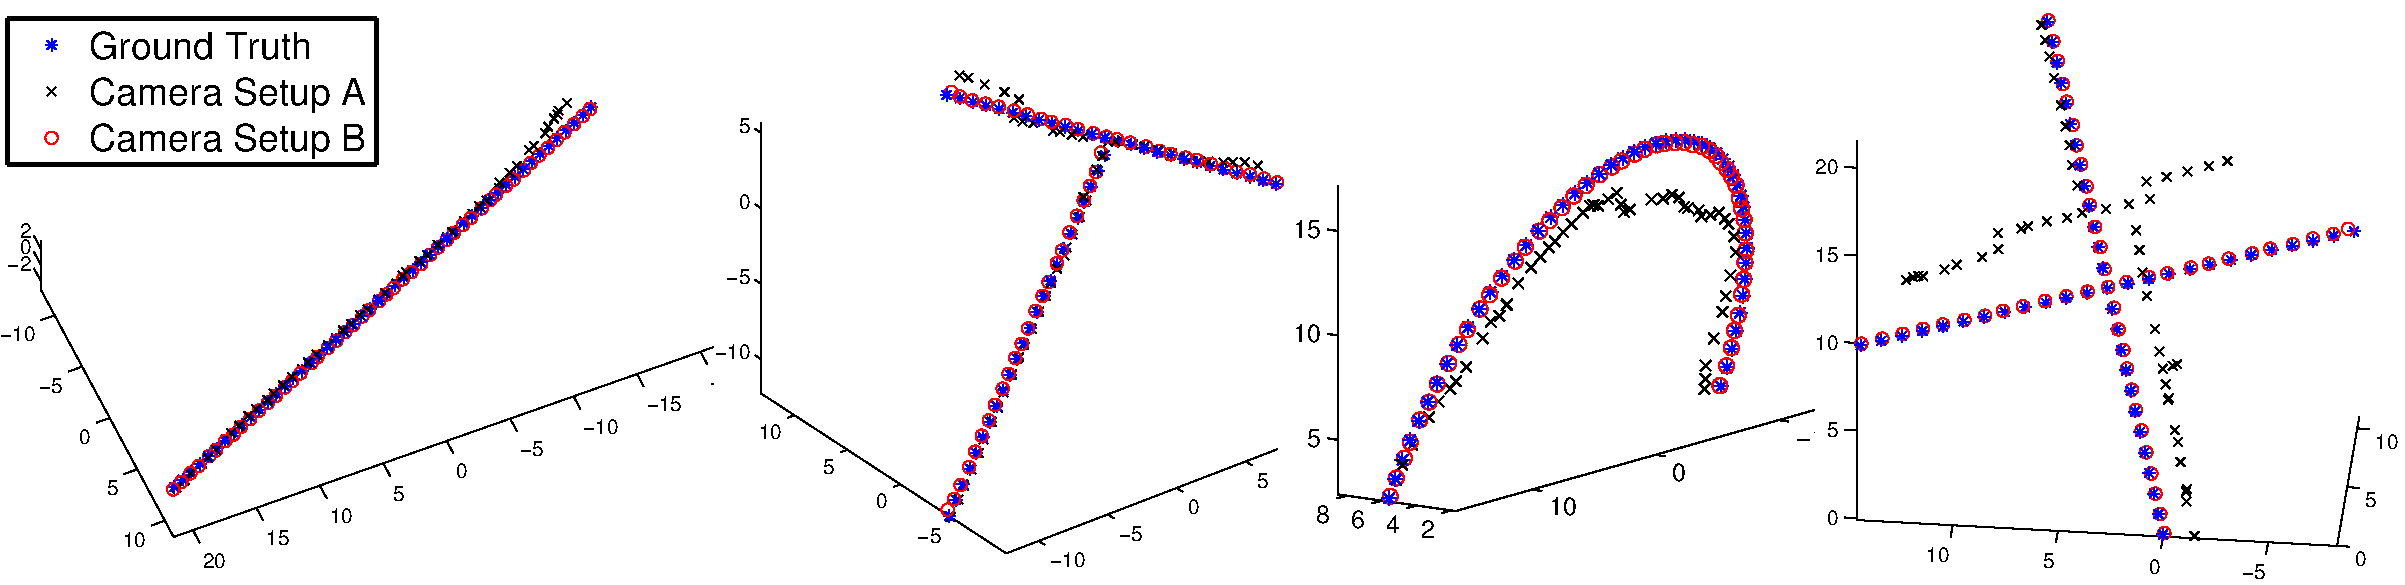
\includegraphics[width=0.98\textwidth]{chapter4/resource/allfig.pdf}
\caption{Example results for line path, T-junction path, half circle and crossed paths.}
\label{fig:synthetic}
\end{figure}


\begin{figure}[t]
\centering
\subfloat{
    \includegraphics[height=0.15\textheight]{chapter4/resource/snapshot03.png}
    }
\subfloat{
    \includegraphics[height=0.15\textheight]{chapter4/resource/snapshot05.png}
    }\\
\subfloat{
    \includegraphics[height=0.18\textheight]{chapter4/resource/tjunction1.PNG}
}
\subfloat{
    \includegraphics[height=0.18\textheight]{chapter4/resource/tjunction2.PNG}
}
\caption{Two views for each of the reconstructed results.}
\label{fig:reconstructed}
\end{figure}

\textbf{Synthetic datasets} Our first experiment uses synthetic data, with six different \oct~shapes on a plane, including a single line path, a T-junction path, a path with two parallel lines, a half circle path, sine wave shaped path, and two crossed path. For each of these shapes, we tested 32 instances, with each containing 50 randomly chosen object observation at different 3D positions. For more convenient error estimation during the evaluation, we normalized the 3D points so that the average distance between every pair of nearest points equals 1. The cameras are randomly generated around the 3D object points with two different configurations. In camera configuration A, all the camera centers stay in the same plane as the 3D points, which is more difficult since each viewing ray may intersect the ground truth path several times. In camera configuration B, the camera centers are set randomly off the plane, with the angle between the viewing ray and the plane being at most $10^\circ$ and camera distance of 2-3 times the length of the path. We choose $k=100$ uniformly distributed discrete 3D hypotheses $\mathbf{X}_i^o$  along each viewing ray $\mathbf{X}_i$ in a range that contains the ground truth 3D point. The size of the range is set as 1.5 times the length of the path. Notice that while the ground truth 3D points lie in the range, it is not guaranteed to be one of the discrete samples $\mathbf{X}_i^o$. %The run time of tGMST algorithm is set 1 hour for each data instance.

Errors are measured using the Euclidean distance between the estimated 3D points and the ground truth. The average errors over the 32 instances for each shape category are listed in Table \ref{fig:syntheticDataResult}. We report errors of the GMST output, and the errors after the continuous refinement using Eq. (\ref{equ:costFunc_continuous}).  Table \ref{fig:syntheticDataResult} shows our  continuous refinement always improves the reconstruction accuracy over the GMST approximation.  The results demonstrate    {\it off-plane} cameras yield improved results than {\it in-plane}  cameras  for  complex paths (e.g. crossed paths), due to the multiplicity of ray-to-path intersections. In these cases the GMST solution has a more complex search space and yields a sub-optimal solution. However, the condition number of the linear system does not vary significantly across configurations. Figure \ref{fig:synthetic} shows the estimated 3D points overlaid onto the ground truth.


\textbf{Real datasets} We evaluated our method on two image datasets  registered by VisualSFM \cite{WuVSFM}. The detection confidence threshold  is set high in order to lower down the false alarm rate. However, a very small amount of false alarms are purged manually as it may affect the reconstruction.  We sample 100 samples along the viewing ray in the range $[0,far]$, where $far$ is  estimated using the model scale. The running time for each object class trajectory is set to 3 hours.

The first dataset captures random pedestrians walking on the sidewalk, and random cars running on a lane. It contains 135 images with 82 valid car detections and 137 valid pedestrian detections. The scene and the reconstructed object class trajectory are shown in Figure \ref{fig:franklin_Recon}. %and the images are taken on the other side of the street at different time.
The second dataset captures several people who are walking on a T-junction shaped path at the corner of a building. It contains 47 images with 66 valid detections. Using the camera positions, we convert the face directions into the global coordinate system to obtain the motion tangents $\mathbf d_i$ of the moving people. For illustration, we construct the background static scene using CMPMVS \cite{JAN}. The general 3D human and car mesh models are inserted into each of the estimated 3D positions. We show different views of the reconstructed results in Figure \ref{fig:reconstructed}.

% show some images, and the results from different views.
%\begin{figure}[t]
%\begin{center}
%\begin{tabular}{|c ||c |c |c| c| }
%\hline
%\includegraphics[width=0.192\textwidth]{chapter4/resource/googlescholar.PNG} &
%\includegraphics[width=0.192\textwidth]{chapter4/resource/cleanFrame083.jpg} & 
%\includegraphics[width=0.192\textwidth]{chapter4/resource/cleanFrame084.jpg} & 
%\includegraphics[width=0.192\textwidth]{chapter4/resource/cleanFrame085.jpg} &
%\includegraphics[width=0.192\textwidth]{chapter4/resource/cleanFrame086.jpg}\\
%\hline
%\includegraphics[width=0.192\textwidth]{chapter4/resource/car_ped_franklin_top.pdf} &
%\includegraphics[width=0.192\textwidth]{chapter4/resource/Frame_083_crop.jpg} & 
%\includegraphics[width=0.192\textwidth]{chapter4/resource/Frame_084_crop.jpg} & 
%\includegraphics[width=0.192\textwidth]{chapter4/resource/Frame_085_crop.jpg} &
%\includegraphics[width=0.192\textwidth]{chapter4/resource/Frame_086_crop.jpg}\\
%\hline
%\end{tabular}
%\end{center}
%\caption{The left column: an aerial image showing the scene and a figure showing the cameras and reconstructed cars and pedestrians. The right four columns: four pedestrian detections (shown in yellow rectangles) and the poses of the corresponding cameras. These four pedestrians are adjacent in the reconstructed object class trajectory. Notice that the second and the third images are the same image but with different detections.}
%\label{fig:franklin_Recon}
%\end{figure}

\begin{figure}[t]
\centering
\begin{tabu}{ |[2pt]c |[2pt] c |[2pt]}
\tabucline[2pt]{-}
\includegraphics[width=0.33\textwidth]{chapter4/resource/googlescholar.PNG} &
\includegraphics[width=0.33\textwidth]{chapter4/resource/car_ped_franklin_top.pdf}  \\
\tabucline[2pt]{-}
\tabucline[2pt]{-}
\includegraphics[width=0.33\textwidth]{chapter4/resource/cleanFrame083.jpg} & 
\includegraphics[width=0.33\textwidth]{chapter4/resource/Frame_083_crop.jpg}  \\
\tabucline[2pt]{-}
\includegraphics[width=0.33\textwidth]{chapter4/resource/cleanFrame084.jpg} &
\includegraphics[width=0.33\textwidth]{chapter4/resource/Frame_084_crop.jpg} \\
\tabucline[2pt]{-}
\includegraphics[width=0.33\textwidth]{chapter4/resource/cleanFrame085.jpg} & 
\includegraphics[width=0.33\textwidth]{chapter4/resource/Frame_085_crop.jpg} \\
\tabucline[2pt]{-}
\includegraphics[width=0.33\textwidth]{chapter4/resource/cleanFrame086.jpg} &
\includegraphics[width=0.33\textwidth]{chapter4/resource/Frame_086_crop.jpg}\\
\tabucline[2pt]{-}
\end{tabu}
\caption{The left row: an aerial image showing the scene and a figure showing the cameras and reconstructed cars and pedestrians. The bottom four rows: four pedestrian detections (shown in yellow rectangles) and the poses of the corresponding cameras. These four pedestrians are adjacent in the reconstructed object class trajectory. Notice that the second and the third images are the same image but with different detections.}
\label{fig:franklin_Recon}
\end{figure}

\section{Conclusions}
We proposed a solution to the novel \jost~problem, which allows the reconstruction of an \oct~from unordered images for which the capture times are unknown and there is no requirement of more than one view observing any object instance. This problem has previously been seen as highly limited in reconstructabililty. We evaluated our proposed method on synthetic and real world datasets and show promising results demonstrating the feasibility of the proposed approach to solve the \jost~problem and in fact the first time demonstrating its solvability.



\input{chapter5/chapter5_}

%%%%%%%%%%%%%%%%%%%%%%%%%%%%%%%%%%%%%%%%%%%%%%%%%%%%%%%%%%%%
%%%%%%%%%%%%%%%%%%%%%%%%%%%%%%%%%%%%%%%%%%%%%%%%%%%%%%%%%%%%
\chapter{Discussion}
\label{ch:discussion}
This dissertation presents three works for the problems in static scene reconstruction and dynamic object reconstruction. In Chapter \ref{ch:patchmatch}, we propose a framework of joint view selection and depthmap estimation. The experiments on large Internet collected photos demonstrates its efficiency and robustness. In Chapter \ref{ch:jost} and Chapter \ref{ch:video_l1}, we solve the problems of dynamic object reconstruction from unstructured images and unsyncthronized videos, respectively. In solving these two problems, our main effort is on 3D reconstruction without sequencing information. We show effectiveness of the approaches by testing on synthetic and real datasets. Next, we discuss the possible extension of our works, and the potential future research directions.

%%%%%%%%%%%%%%%%%%%%%%%%%%%%%%%%%%%%%%%%
\section{Future work}

%%%%%%%%%%%%%%%%%%%%%%%%%%%%%%%%%%%%%%%%
\subsection{Extensions to PatchMatch-based joint view selection and depthmap estimation}
\label{sec:patchmatch_extensions}

Though our method significantly outperforms existing methods on Internet collected photos \cite{Goesele07}, and achieves the state-of-the-art accuracy on standard datasets collected under controlled lab environment \cite{Strecha08}. The accuracy of the method can be further improved by incorporating some standard techniques into our framework. Next, we discuss each of the techniques for possible accuracy improvement.

In the method, we use the frontal-parallel planes to warp color patches into other images for color consistency check. It has been shown the plane orientation affects the reconstruction accuracy \cite{Gallup07,FURUKAWA_PAMI2010}. Ideally, the plane orientation should be close to the real surface normal, which is unknown before reconstruction. To address this issue, the surface normal can be included as unknown variables in our framework. Specifically, the normal directions are propagated to the neighboring pixels in addition to the depth \cite{patchMatchStereo1}. This scheme has a potential to further improve reconstruction quality on the regions having large angles with the camera viewing directions (e.g. the ground), but increases the computation complexity.

Another issue relating to the color patch arises if the pixels in a patch cover scenes of significantly different depths, which typically occurs at the boundary of object surfaces. 
When compare color consistency between two pixels, current local methods (\ie no smoothness term in the depthmap) use the whole patches around the pixels to improve the robustness.
The method present in Chapter \ref{ch:patchmatch} uses NCC as a metric to measure the color consistency, where each pixel in the patch contributes equally for the measure.
However, this is likely to produce swollen/fat boundaries in the depthmap, since the usage of a plane for patch warping assumes all pixels in the patch have the same depth and normal, and this assumption breaks at the boundary of object surfaces. Therefore, when measuring the color consistency between two patches, the pixels with the same depth as the central pixel should be given more weights than other pixels. To achieve this, one effective solution is using adaptive weights for each pixel in the patch based on color similarity and geometric proximity relative to the central pixel \cite{Yoon06adaptivesupport_weight}. 

Another extension to our work is to handle cameras with small baselines. In stereo methods, small baselines usually lead to unstable and inaccurate results. Since the large set of Internet collected photos is typically taken at certain spots of interest, it is very likely some of the images have very small or zero baselines. Our framework select images based on color consistency, and the images with small baselines will be selected since the color consistency are always good regardless of estimated depth. To address this issue, the angles of two viewing rays given a depth hypothesis should be computed to prevent invalid triangulation \cite{Gallup08}. Specifically,when estimating the depth of a pixel, if the angle of two viewing rays is below a threshold, the corresponding source image is eliminated.

Though great advance in depth estimation has been achieved, there are still some important problems remain unsolved. One case in point is depth estimation for homegenerous color regions. 
Most current methods estimate depth by checking color consistency, and none of them can successfully address this issue.  
To handle this problem, I believe it is necessary to incorporate the semantic knowledge of the scene rather than to just rely on low-level colors. This inevitably requires introducing the machine learning techniques into stereo problems. However, the incorporation of camera parameters into machine learning frameworks has another issue, since the testing data and training data may have different camera parameters. Though there are many single image depth estimation based on supervised machine learning \cite{Hoiem_CGRAPH2005,Saxena_IJCV2008,eigen2014depth,Liu2014,zhuo2015indoor}, incorporating this technique into multiview stereo methods for accurate depth estimation still has long way to go.

%%%%%%%%%%%%%%%%%%%%%%%%%%%%%%%%%%%%%%%%
\subsection{Extensions to JOST}

The method presented in Chapter \ref{ch:jost} uses object detection output as features, and the object lies along the viewing ray passing the features. However, our method cannot handle outlier detection (false alarm), and the outliers may stop the method from finding the correct trajectory. One way to manage this problem, as is done in the paper, is to raise the detection threshold to suppress the false alarm rate (at the cost of increasing miss detection). Another possible way is to embed our method in a RANSAC framework \cite{Hartley2004} to remove outliers. Specifically, the subset of sampled detections is used to triangulate the trajectory, and count the number of remaining detections censuses with the trajectory (\ie~inliers). Repeat this process to find the trajectory with the largest number of inliers. However, this scheme is computational intensive if the ratio of outliers is large, considering that running trajectory triangulation given  a subset of detections is time-consuming. 

Efficiency is another issue for our approach. In our method, the nonconvex problem is solved in a discrete-continuous scheme, and the discrete step involves solving a NP-hard GMST problem. The efficiency of solving a GMST problem can be attained by reducing the complexity of the K-partite graph. A complete K-partite graph has all the nodes in one set connecting to all the nodes in another set. The computation complexity of GMST given the graph will be lowered down if the number of edges and nodes is reduced. To simplify the K-partite graph, if given a prior knowledge that two specific detected objects are farther away in 3D space, then all the edges connecting the associated two sets of nodes can be safely removed. Moreover, the size of each object detection window can be used to roughly estimate the tight depth range of the dynamic object, which helps reduce the size of each node set and hence the number of edges.

\subsection{Extensions to dynamic object reconstruction from unsynchronized videos}

The method presented in Chapter \ref{ch:video_l1} requires a static background scene present in the image so that structure from motion can use it for camera registration. However, the crowd sourced data may have the dynamic object as main focus and lack the content of the background scene. This comes an open question of how to register cameras given non-current captures of dynamic objects. Considering the importance and difficulity of this problem, it can be a possible future research direction.

Moreover, to the best of our knowledge, the work is the first self-representation framework for dynamic object reconstruction. That is, each temporal shape can be represented by a linear combination of a few other shapes given the smooth motion of dynamic objects. This self-representation constraint has potential to be applied in the NRSFM problems. Comparing to most of the existing works, where the assumption that any shape is a linear combination of $K$ shape bases is applied, our self-representation constraint is more intuitive and possibly lead to better reconstruction results.

% obtaining correspondences.
% possible dense reconstruction.





















% Bibliography
% !TEX root = ../thesis_heinly.tex

\clearpage
\phantomsection

{\def\chapter*#1{} % suppress bibliograph header.
\begin{singlespace}
\addcontentsline{toc}{chapter}{BIBLIOGRAPHY}
\begin{center}
\textbf{BIBLIOGRAPHY}
\vspace{20pt}
\end{center}

\bibliographystyle{apalike}
\bibliography{bibliography}
\end{singlespace}
}


\end{document}
